%%%%%%%%%%%%%%%%%%%%%%%%%%%%%%%%%%%%%%%%%
% Masters This 
%
% Thesis template is based on templates by:
% - Mario Román (https://github.com/mroman42)
% - Steve Gunn (http://users.ecs.soton.ac.uk/srg/softwaretools/document/templates/)
% - Sunil Patel (http://www.sunilpatel.co.uk/thesis-template/)
%
% Modifications done by Pedro Bonilla. 
% Template license:
% CC BY-NC-SA 3.0 (http://creativecommons.org/licenses/by-nc-sa/3.0/)
%
%%%%%%%%%%%%%%%%%%%%%%%%%%%%%%%%%%%%%%%%%

%----------------------------------------------------------------------------------------
%	PACKAGES AND OTHER DOCUMENT CONFIGURATIONS
%----------------------------------------------------------------------------------------

\documentclass[
11pt,
% oneside, % Two side (alternating margins) for binding by default, uncomment to switch to one side
english, % ngerman for German
singlespacing, % Single line spacing, alternatives: onehalfspacing or doublespacing
%draft, % Uncomment to enable draft mode (no pictures, no links, overfull hboxes indicated)
%nolistspacing, % If the document is onehalfspacing or doublespacing, uncomment this  to set spacing in lists to single
%liststotoc, % Uncomment to add the list of figures/tables/etc to the table of contents
%toctotoc, % Uncomment to add the main table of contents to the table of contents
%parskip, % Uncomment to add space between paragraphs
%nohyperref, % Uncomment to not load the hyperref package
headsepline, % Uncomment to get a line under the header
%chapterinoneline, % Uncomment to place the chapter title next to the number on one line
%consistentlayout, % Uncomment to change the layout of the declaration, abstract and acknowledgements pages to match the default layout
]{MastersDoctoralThesis} % The class file specifying the document structure


\usepackage[utf8]{inputenc} % Required for inputting international characters
\usepackage[T1]{fontenc} % Output font encoding for international characters
\usepackage{stmaryrd}
\usepackage{mathpazo} % Use the Palatino font by default
\usepackage[font=itshape]{quoting} 
\usepackage[toc,page]{appendix}
\usepackage{pdfpages}
\usepackage[backend=biber,style=numeric]{biblatex} 
\usepackage[activate={true,nocompatibility},final,tracking=true,kerning=true,spacing=true,factor=1100,stretch=10,shrink=10]{microtype}
\usepackage{eso-pic}
\usepackage[autostyle=true]{csquotes} 


\newenvironment{sproof}{\renewcommand{\proofname}{Sketch Proof}\proof}{\endproof}

\addbibresource{./example.bib} % The filename of the bibliography


% ----------------------------------------------------------------------------------
%	MARGIN SETTINGS
%----------------------------------------------------------------------------------

\geometry{
	paper=a4paper, % Change to letterpaper for US letter
	inner=2.5cm, % Inner margin
	outer=3.8cm, % Outer margin
	bindingoffset=.5cm, % Binding offset
	top=1.5cm, % Top margin
	bottom=1.5cm, % Bottom margin
	%showframe, % Uncomment to show how the type block is set on the page
}

%----------------------------------------------------------------------------------
%	THESIS INFORMATION AND METADATA
%----------------------------------------------------------------------------------
\usepackage[allcolors=myred]{hyperref}

\author{Pedro Bonilla Nadal}
\newcommand{\miTitulo}{Dependent Typing through Closed Cartesian Categories\\\xspace}
\newcommand{\miNombre}{Pedro Bonilla Nadal\xspace} 
\newcommand{\miGrado}{Máster en Matemáticas y Aplicaciones}
\newcommand{\miFacultad}{Facultad de Ciencias}
\newcommand{\miUniversidad}{Universidad Autónoma de Madrid}
% Añadir tantos tutores como sea necesario separando cada uno de ellos
% mediante el comando `\\\medskip` y una línea en blanco
\newcommand{\miTutor}{
Dr. Ángel González Prieto  \\ \emph{Departamento de Matemáticas \\ Universidad Autónoma de Madrid}}
\newcommand{\miCurso}{2020-2021\xspace}
\newcommand{\misPalabrasClave}{HOTT, McLane}
\newcommand{\K}{\mathbb{K}}


\hypersetup{pdfinfo={
            Title={\miTitulo},
            Author={\miNombre},
            Director1={Dr. Ángel González Prieto},
            Ndirectores={1}
            Tipo={TFM},
            Curso={\miCurso},
            MSC={ MSC2020},
            Palabrasclave={\misPalabrasClave},
          }
        }

\AtBeginDocument{
\hypersetup{pdftitle=\miTitulo} 
\hypersetup{pdfauthor=\miNombre}
\hypersetup{pdfkeywords=\misPalabrasClave}
}

%%%%%%%%%%%%%%%%%%%%%%%%%%%%%%%%%%%%%%%%%%%%%%%%%%%%%%%%%%%%%%%%%%%%%%%%%%%%%%%%%%%


%----------------------------------------------------------------------------------
%          OTHER IMPORTS
%----------------------------------------------------------------------------------


\usepackage{titlesec}


%\usepackage[british]{babel}
\usepackage{caption}
\usepackage{adjustbox}
\usepackage{enumitem}
\usepackage{boldline}
\usepackage{amssymb, amsmath}
\usepackage{amsthm}
\usepackage{soul}
\usepackage{upgreek}
\usepackage{wrapfig}
\usepackage{mathtools}
\usepackage{epigraph}
\usepackage{algorithm}
\usepackage[noend]{algpseudocode}
\usepackage{soul}
\usepackage{graphicx}
\usepackage{mathrsfs}
\usepackage{xcolor}
\usepackage{listings}
\usepackage{tikz-cd}

\tikzcdset{arrow style=tikz, diagrams={>=stealth}}

\newtheorem{theorem}{Theorem}[section]
\newtheorem{corollary}{Corollary}[theorem]
\newtheorem{thesis}[theorem]{Thesis}
\newtheorem{lemma}[theorem]{Lemma}
\theoremstyle{definition}
\newtheorem{definition}{Definition}[section]
\newtheorem{proposition}{Proposition}[section]
\newtheorem{example}{Example}[section]
\newtheorem{remark}{Remark}[section]
\newcommand\myeq{\stackrel{\mathclap{\normalfont\mbox{?}}}{=}}

\newcommand{\R}{\mathbb{R}}
\newcommand{\N}{\mathbb{N}}
\newcommand{\dom}{\operatorname{dom}}
\newcommand{\colim}{\operatorname{colim}}
\newcommand{\codom}{\operatorname{codom}}
\newcommand{\hhom}{\operatorname{hom}}
\newcommand{\maybe}{\operatorname{Maybe}}
\newcommand{\oo}{\operatorname{ or }}
\newcommand{\ccase}{\operatorname{case}}
\newcommand{\iin}{\operatorname{in}}
\newcommand{\LL}{\mathcal{L}}
\newcommand{\LC}{\lambda\operatorname{Calc}}


\begin{document}
\frontmatter

\includepdf{img/portada.pdf}
\cleardoublepage
% !TeX root = ../libro.tex
% !TeX encoding = utf8

%*******************************************************
% Little Dirty Titlepage
%*******************************************************

\thispagestyle{empty}

\begin{center}
  {\small TODO: incluir portada oficial}
  \large  

  \vspace*{\stretch{1}}

  \begingroup
  \huge{\miTitulo} \\
  {\small (Título provisional - busca uno definitivo - probablemente en mayo)}
  \bigskip
  
  \endgroup

  \textrm{\miNombre}

  \vspace{\stretch{5}}

\end{center}  

\newpage
\thispagestyle{empty}

\hfill

\vfill

\miNombre\ \textit{\miTitulo}.

Master's thesis.

Academic year \miCurso.\\

\begin{minipage}[t]{0.25\textwidth}
  \flushleft
  \textbf{Thesis\\ supervisor}
\end{minipage}
\begin{minipage}[t]{0.40\textwidth}
  \flushleft
  \miTutor
\end{minipage}
\begin{minipage}[t]{0.35\textwidth}
  \flushright
  \miGrado
  \medskip

  \miUniversidad
\end{minipage}
\begin{flushleft}
\end{flushleft}

\endinput

% % !TeX root = ../libro.tex
% !TeX encoding = utf8
%
%*******************************************************
% Declaración de originalidad
%*******************************************************

\thispagestyle{empty}

\hfill\vfill

\textsc{Statement of Originality}\\\bigskip

D. \miNombre \\\medskip

 
I explicitly declare that the work presented as a Master's thesis (TFM) corresponding to the academic year \miCurso, is original, understood in the sense that it has not used sources for the elaboration of the work without citing them properly.

\medskip

Madrid, \today.
\begin{flushleft} 
Fdo: \miNombre 

\end{flushleft}

\vfill

\cleardoublepage
\endinput

% % !TeX root = ../libro.tex
% !TeX encoding = utf8

%*******************************************************
% Dedication
%*******************************************************
\thispagestyle{empty}
\phantomsection 
\pdfbookmark[1]{Dedicatoria}{Dedicatoria}

\hfill
\vfill

\begin{flushright}
\itshape
Una dedicatoria a una persona probablemente.
\end{flushright}

\vfill

\cleardoublepage
\endinput

\pagestyle{thesis}
{
  \hypersetup{hidelinks}
  \setcounter{tocdepth}{2}
  \tableofcontents
}
% %*******************************************************
% Introducción
%*******************************************************

% \manualmark
% \markboth{\textsc{Introducción}}{\textsc{Introducción}} 
\chapter{Introduction}


The great revolution in mathematics, already started in the middle of the 19th century with the epsilon-delt formalism, is the formalization of mathematics. During this period, brilliant mathematicians Weierstrass, Hilbert and most notably the group  Bourbaki put formalism at the core of mathematics. \\

Of all the areas that benefited from formalization, computation was probably the one that came out best. After the work of Church and Turing it became the mathematical element that would most seriously transform the world, like a steam engine of the contemporary era.This transformation was so radical that a person 50 years ago would not understand how to use the tools with which the population spends more than half of its waking hours.\\

The aim of this work is thus to strain the world-transforming idea of computation into an algebraic theory. This work  adopts a slow but steady pace, for before being able to strain one must first know how to use the straining tools, and then know in depth what one intends to strain.  \\

After the work of previous mathematicians such as Galois and Poincare, and in view of the new formalization and organization of mathematics, mathematicians such as MacLane, Elineberg, Cartan or Grothendiek began to form and expand what we know today as category theory. This theory effectively strained mathematical ideas in their purest form, and generate theories seemingly ubiquitous. After all, we study category as a knowledge condenser.\\

In the first part of this paper we will talk about the theory of categories, explaining and introducing it. In the second part of the paper, we will navigate in the concept of lambda calculus, as the first formalizing idea of computation. Both theories will be introduced with the point of view of the person who is interested in only one of them.\\

It is in the third part when the pairing happens. In particular the fourth chapter we raise all the bridges between closed Cartesian categories and computation with types. Finally, in chapter 5, we use ideas with the same flavor to prove a similar equivalence with Martin-L\"of's theories. \\

Thus, this paper will deal with the intuition behind the formalism. We encourage the reader to try to gain in his reading an idea, not only formal but intuitive, of what computation is, and what lies at the heart of this idea.  After all, in the immortal words of Karl Weierstrass \cite{duporcq1902compte}

\begin{quote}
... it is true that a mathematician who is not somewhat of a poet, will never be a perfect mathematician.\\
\end{quote}

\section*{Main goals and results achieved}
The initials goals of this thesis were:
\begin{enumerate}
\item Accomplish a theoretical study of the foundations of category theory.
\item Accomplish a theoretical study of the foundations of $\lambda$-calculus and typing theory.
\item Unify both point of view after the works of Lambek \cite{lambek1988introduction} and Seely \cite{seely1984locally}.
\end{enumerate}

We consider that both three objectives have been accomplish successfully.\\

We also consider the work of a particular interest, because instead of making an introduction of the concepts of category and typing more given to the later proof of equality, we prefer to work with the concepts in the form where their intuitive notion is clearer, in the formulation that mathematicians whose objective is the study of each area and not its pairing with each other.



\endinput
               
% \begin{otherlanguage}{spanish}
%   %*******************************************************
% Summary
%*******************************************************

\newpage



\chapter*{Summary}
\addcontentsline{toc}{chapter}{Summary}
\section*{Brief Summary}

English Abstract

\textbf{keywords:} 



\selectlanguage{spanish}
\section*{Resumen Extendido}

Resumen extendido en español

\textbf{palabras clave:} 


\selectlanguage{english}


% \endinput
                    
% \end{otherlanguage}

\mainmatter
\part{Category Theory}
\thispagestyle{empty}
\label{Part1}

\part{Category Theory}
\label{Part1}



\chapter{First Notions of Category Theory}

%%%%%%%%%%%%%%%%%%%%%%%%%%%%%%%%%%%%%%%%%%%%%%%%%%%%%%%%%%%%%%%%%%%%%%%% 
\epigraph{“The human mind has never invented a labor-saving machine equal to algebra.” }{\textit{Stephan Banach (1925)}}

For us, Categories are an area of interest on its own rights, rather than merely an elegant tool. In this sense we will introduce this theory with a personal point of view, trying to emphasize the intuitive ideas behind each notion.\\

Thus, in addition to the formal content, we will also provide enough information so that an avid reader gain quick intuitive understanding of the subject. With this objective in mind, we will get into the habit of introducing the first examples even before introducing the formal definitions. Thus, when the formal definition is introduced, it becomes more meaningful and helps the intuition to understand the concept.\\

The fundamental idea of Category Theory is that a many properties can be unified if expressed with diagram and arrows. Intuitively, a diagram is a directed graph, such that each way of going from a node to another are equals. For example, in the diagram:

\[
  \begin{tikzcd}
    & b \arrow[rd, "g"]& \\
    a\arrow[ru, "f"] \arrow[rr, "h"] && c\\
  \end{tikzcd}
\]
Means that $f\circ g = h$. This approach to mathematics emphasises  at the relationships between elements, rather than at the elements themselves (and from them derive their relationships).\\

In this first chapter we will introduce the notion of category and their first properties. The principal references for this chapter are \cite{mac2013categories} and \cite{riehl2017category}. 

\section{Metacategories}
We will start by defining a concept independent of the set theory axioms: the concept of \emph{metacategory}. Once this is done we will follow reinterpreting this definitions in the context of set theory. We define categories following  \cite{mac2013categories}.\\


Traditionally, mathematics is based on the set theory. When we start set theory it is not necessary (it is not possible) to define what a set is. It is similar with the concepts of element and belonging, which are basic to set theory. Category theory can also be used to found mathematics. In this sense we will give definitions based on other concepts such as object, arrow, composition. \\

\begin{definition}
  A \emph{metagraph} consist of \emph{objects}: $a,b,c..$ and \emph{arrows} $f,g,h...$. There are also two pairings: $\dom$ and $\codom$. This pairings assigns each arrow with an object. An arrow $f$ with $\dom(f)=a$ and $\codom(f)=b$ is usually denoted as $f:a\to b$.\\
\end{definition}

\begin{definition}
  A metacategory  is a metagraph with two additional operations:
  \begin{itemize}
  \item \emph{Identity}: assigns to each object $a$ an arrow $1_a:a\to a$. 
  \item \emph{Composition}: assigns to each pair of arrows $f,g$ with $\codom(f)=\dom(g)$ and arrow $g\circ f$ such that the diagram:

    \[
      \begin{tikzcd}
        & b \arrow[rd, "g"]& \\
        a\arrow[ru, "f"] \arrow[rr, "g\circ f",swap] && c\\
      \end{tikzcd}
    \]

    commutes. The arrow $g\circ f$ is called the \emph{composite} of $f$  and $g$.
  \end{itemize}

  There are additional two properties:
  \begin{itemize}
  \item \emph{Associative}: given arrows $f,g,h$, we have that,
    $$(g\circ f) \circ h = g \circ (f \circ h).$$
  \item \emph{Unit}: given an object $a$, and arrows $f,g$ such that $\dom (f)= a$ and $\docom (g) = a$, we have that,
    $$1_a \circ g = g, \qquad f \circ 1_a = f.$$
  \end{itemize}
  In the context of a metacategory, arrows are often called \emph{morphisms}.
\end{definition}

We have just define what a  metacategory is without any need of set and elements. In most cases we will rely in a set theory interpretation of this definitions, as most examples will rely on this theory. Nonetheless, whenever possible, we will define the concepts working only in terms of objects and arrows, having therefore the theory as independent as possible to this theory.

% Diagramas de existencia condicionada.!!
% We will also need diagrams that represents the existence of arrows due to the existence other arrows. , given objects $a,b,c$ and arrows $d$



\section{ZFC Axioms}
{\color{red}(Maybe) TODO}: Introduce fundamental terminology and problems related to classical set theory.\\

Once we have talk so much about this we may also formally introduce the stuff. Is not so long (?)  - ok, maybe it is. I am letting this as a TODO and continue with other stuff until this is more done.\\

Further on i left a detailed todo of things from this section that are referenced in the text.\\

Detailed TODO:
\begin{itemize}
\item small sets and large sets.
\end{itemize}


\section{Set theory categories}
Further on we will work based on set theory.

\begin{definition}
  A category (resp. graph) is an interpretation of a metacategory (resp. metagraph) within set theory.
\end{definition}


That is, a graph/category is a pair $(O,A)$ where a set $O$ consisting of all objects as well as a set $A$ consisting of all arrows. Their elements holds the same properties that objects and arrows satisfy on metacategories / metagraph.\\


We will focus on the category. We can also define the function homeset of a category $C=(O,A)$, wrote as $\hom_{C}$, as the function:
\begin{align*}
  && \hom_{C}: O \times O &\mapsto \mathcal{P}(A)&\\
  \displaystyle &\ &(a,b)&\mapsto \{f\in A | f:a\to b\}&
\end{align*}

With this definitions done, we will carry on working on examples and properties of the categories.

\begin{definition}
  We say that a category is \emph{small} if the collection of objects is given by a set (instead of a proper class). We say that a category is \emph{locally small} if every homesets is a set.
\end{definition}

\subsection{Examples\footnote{Debería cambiar esto por un entorno de ejemplo grande?}}
We proceed to introduce a comprehensive list of examples, so that it is already introduced in subsequent chapters.

\begin{itemize}
\item The ``example'' category:
  \begin{itemize}
  \item The category $0 = ( \emptyset, \emptyset)$ where every property is trivially satisfy.
  \item The category $1 = (\{e\},\{1_e\})$.
  \item The category $2 = (\{a,b\},\{1_a,1_b,f:a\to b\})$
  \end{itemize}

\item Discrete categories: are categories where every arrow is an identity arrow. This are sets regarded as categories, in the following sense: every discrete category $C=(A, \{1_a : a \in A\})$ is fully identified by its set of object.  
\item Monoids and Groups: A monoid is a category with one object (regarding the monoid of the arrows). In the same way, if we requires the arrows to satisfy the inverse property, we can see a group as a single-object category. 
\item Preorder: From a preorder $(A, \le)$ we can define a category $C = (A, B)$ where $B$ has an arrow $e: a \to b$ for every $a,b\in A$ such that $a \le B$. The identity arrow is the arrow that arise from the reflexive property of the preorders. 

\item Large categories: these categories has a large set of objects. For example:
  \begin{itemize}
\item The category $Top$ that has as objects all small topological spaces and as arrow continuous mappings.
\item The category $Set$ that has as objects all small sets and as arrows all functions between them.
\item The category $Vect$ That has as object all small vector spaces and as arrows all linear functions.
\end{itemize}

\item Include more examples as categories are used in the text.
\end{itemize}

Note that, for example,  as natural numbers can be seen as either a set or a preorder, they also can be seen as a discrete category or a preorder category.




\subsection{Some properties on arrows}
\subsubsection{Equality}
We can see that is common in mathematics to have an object of study (propositional logic clauses, groups, Banach spaces or types in Haskell). Once the purpose of the study of these particular set of objects is fixed, it is also common to proceed to consider the transformations between these objects (partial truth assignments, homomorphisms, linear bounded functionals or  functions in Haskell).\\

In categories, we have a kind of different approach to the subject. Instead of focusing in the objects themselves, we focus on how they relate to each other. That is, we focus on the study of the arrows and how they composes. Therefore we can consider equal two objects that has the same relations with other objects. This inspire the next definition:

\begin{definition}[definition 1.1.9 \cite{riehl2017category}]
  Given a category $C=(O,A)$, a morphism $f: a \to b \in A$ has a \emph{left inverse} (resp. \emph{right inverse}) if there exists a $g: b \to a \in A$ such that $g \circ f = 1_b$ (resp. $f \circ g = 1_a$). A morpishm is an isomorphism if it has both left and right inverse, called the \emph{inverse}. 
\end{definition}

%Given a category $C=(O,A)$, an \emph{isomorphism} is a morphism $f: a \to b \in A$ for which there exists $g: b\to a\in A$ such that $f\circ g = 1_a$ and $g \circ f = 1_b$.  \\


Is easy to follow that this functions define bijections between $\hom(a,c)$ and $hom(b,c)$ para todo $c\in O$. Also one can see that if a morphism has a left and a right inverse, they must be the same, thus implying the uniqueness of the inverse.

\subsubsection{Special arrows}
\begin{itemize}
\item monics, epics and zeros.
\end{itemize}

\subsubsection{Duality}

Let $C = (O,A)$ be a category. Then, we can define another category $C' = (O,A')$ where we change the domain with the codomain and viceversa. 

\subsection{Transformation in categories}




\subsubsection{Functors}
This is one of the main ways of defining a category: consider a collection of objects and the standard way of transforms one into each other. Then, we may also follow our study defining the structure preserving transformation of categories.

\begin{definition}
  Given two categories $C=(C_O, C_A), B=(B_O, B_A)$, a \emph{functor} $F: B \to C$ is a pair of functions $F=(F',F'')$ (the \emph{object function} and the \emph{arrow functor} respectively)  such that if $g:a\to b \in B_A$ then $F''g$ is an arrow in $C_A$ from $F'a$ to $F'b$.

\end{definition}

That is a functor is a morphism of categories. When there is no ambiguity we will represent both $F'$ and $F''$ with a single symbol $F$ acting on both objects and arrows. Also, as you can see in the definition, whenever possible the parentheses of the functor will be dropped.\\

We can now construct the category of all small categories $Cat$. This category has as object all small categories and as arrows all functor between them. Note that $Cat$ does not contain itself.\\


is left to include:
\begin{itemize}
\item full, lluf, faithfull functor.
\item 
\end{itemize}
\subsubsection{Contravariance}


\subsubsection{Natural Transformations}


\subsection{Some constructions}
\begin{itemize}
\item
\end{itemize}


\chapter{Functors and Natural Transformation}
\section{Definition}
$$
\begin{tikzcd}[row sep = 1.4cm, column sep = 1.4cm]
  F(c)
  \arrow[lddr, to path= { --
    ([xshift=-1ex]\tikztostart.west)
    -| ([xshift=-2ex]\tikztotarget.west)
    |- (\tikztotarget)}]
  \arrow[d, swap, "\sigma(c)"]
  \arrow[r, "F(f)"] 
  & F(c')
  \arrow[d, "\sigma(c')"]
  \arrow[rddl, to path= { --
    ([xshift=1ex]\tikztostart.east) 
    -| ([xshift=2ex]\tikztotarget.east)
    -- (\tikztotarget)}, "\sigma \circ \tau(c')"]
  \\
  G(c)
  \arrow[d, swap, "\tau(c)"] 
  \arrow[r, "G(f)"] & G(c')
  \arrow[d, "\tau(c')"] \\
  H(c) 
  \arrow[r, "H(f)"] & H(c')
\end{tikzcd}
$$
\subsection{Bifunctors}
\subsubsection{The $Hom(\cdot,\cdot)$ bifunctor}
\section{Universality}
In this section we present the concept of universality. This concept is behind lots of mathematical properties. Intuitively, universality is an efficient way of expressing an one-to-one correspondence between arrows of different categories. This one-to-one relationship is usually expressed via ''given an arrow  $y$ it exists one and only one  arrow $x$ such that <insert your favorite universality property''.\\

Prior to the formal definition, we shall introduce an example. Probably the first contact that any mathematician has with universality is when we first try to define a function  $f:\mathbb R \to \mathbb R^2$. We quickly understand that defining such a function is equivalent to define two $g,h: \mathbb R \to \mathbb R$( we further explain the product in \ref{prod-univ} ). Another example is given when you consider the space quotient of a set A for a $~$ relationship over it. In this case, giving a function from $A/~$ is the same as giving a function from $A$ that maintains the equivalence relationship $a~b \implies f(a)=f(b)$. A similar concept lays for almost every quotient structure. Here is the general concept.

\begin{definition}
  If $S: D \to C$ is a functor and $c$ an object of $C$, a universal arrow such that from $c$ to $S$ is a pair $<r,u>$ with $r\in D, u \in Ar(C)$, such that the diagram:
  \[
    \begin{tikzcd}
      & b \arrow[rd, "g"]& \\
      a\arrow[ru, "f"] \arrow[rr, "h"] && c\\
    \end{tikzcd}
  \]

  commutes. 
\end{definition}

\subsection{Yoneda's lemma}
Yoneda's lemma is one of the main results of category theory. This results is due to japanese professor Nobuo Yoneda. We know about Yoneda's life thanks to the elegy that was written by Yoshiki Kinoshita\cite{yonedaLife}. Yoneda was born in Japan in 1930, and received his doctorate in mathematics from Tokyo University in 1952. He was a reviewer for international mathematical journals. In addition to his contributions to the field of mathematics, he also devoted his research to computer science.\\

Mac Lane\cite{mac2013categories} assures the lemma first appeared in his private communication with Yoneda in 1954. With time, this result has became one of the most relevant. The idea behind the Yoneda's lemma is better understood in the context of Moduli problems. 

\subsubsection{Statement and proof}

\subsubsection{The Yoneda's Embedding}
We can easily see that 


\subsection{Some properties expressed in terms of universality}
We can see that the Yoneda lemma provide an embedding form 

\begin{itemize}
\item product \label{prod-univ}
\end{itemize}
\section{Adjoints}


\section{Monad}

\chapter{Unnamed chapter}
\section{Definition}
% $$
% \begin{tikzcd}[row sep = 1.4cm, column sep = 1.4cm]
%   F(c)
%   \arrow[lddr, to path= { --
%     ([xshift=-1ex]\tikztostart.west)
%     -| ([xshift=-2ex]\tikztotarget.west)
%     |- (\tikztotarget)}]
%   \arrow[d, swap, "\sigma(c)"]
%   \arrow[r, "F(f)"] 
%   & F(c')
%   \arrow[d, "\sigma(c')"]
%   \arrow[rddl, to path= { --
%     ([xshift=1ex]\tikztostart.east) 
%     -| ([xshift=2ex]\tikztotarget.east)
%     -- (\tikztotarget)}, "\sigma \circ \tau(c')"]
%   \\
%   G(c)
%   \arrow[d, swap, "\tau(c)"] 
%   \arrow[r, "G(f)"] & G(c')
%   \arrow[d, "\tau(c')"] \\
%   H(c) 
%   \arrow[r, "H(f)"] & H(c')
% \end{tikzcd}
% $$
\section{Universality}
In this section we present the concept of universality. This concept is behind lots of mathematical properties. Intuitively, universality is an efficient way of expressing an one-to-one correspondence between arrows of different categories. This one-to-one relationship is usually expressed via ''given an arrow  $y$ it exists one and only one  arrow $x$ such that <insert your favorite universality property''.\\

Prior to the formal definition, we shall introduce an example. Probably the first contact that any mathematician has with universality is when we first try to define a function  $f:\mathbb R \to \mathbb R^2$. We quickly understand that defining such a function is equivalent to define two $g,h: \mathbb R \to \mathbb R$( we further explain the product in \ref{prod-univ} ). Another example is given when you consider the space quotient of a set A for a $~$ relationship over it. In this case, giving a function from $A/~$ is the same as giving a function from $A$ that maintains the equivalence relationship $a~b \implies f(a)=f(b)$. A similar concept lays for almost every quotient structure. Here is the general concept.

\begin{definition}
  If $S: D \to C$ is a functor and $c$ an object of $C$, an \emph{universal arrow} at from $c$ to $S$ is a pair $<r,u>$ with $r\in D, u \in Ar(C)$, such that the diagram:
  \[
    \begin{tikzcd}
      & b \arrow[rd, "g"]& \\
      a\arrow[ru, "f"] \arrow[rr, "h"] && c\\
    \end{tikzcd}
  \]

  commutes. 
\end{definition}

\subsection{Yoneda's lemma}
Yoneda's lemma is one of the main results of category theory. This results is due to japanese professor Nobuo Yoneda. We know about Yoneda's life thanks to the elegy that was written by Yoshiki Kinoshita\cite{yonedaLife}. Yoneda was born in Japan in 1930, and received his doctorate in mathematics from Tokyo University in 1952. He was a reviewer for international mathematical journals. In addition to his contributions to the field of mathematics, he also devoted his research to computer science.\\

Mac Lane\cite{mac2013categories} assures the lemma first appeared in his private communication with Yoneda in 1954. With time, this result has became one of the most relevant. The idea behind the Yoneda's lemma is better understood in the context of Moduli problems. 

\subsubsection{Statement and proof}

\subsubsection{The Yoneda's Embedding}
We can easily see that 


\subsection{Some properties expressed in terms of universality}
We can see that the Yoneda lemma provide an embedding form 

\begin{itemize}
\item product \label{prod-univ}
\item pullback: dejo estos dibujos muy convenientes guardados.
  $$
\begin{tikzcd}
Q
\arrow[bend left]{drr}{q_2}
\arrow[bend right,swap]{ddr}{q_1}
\arrow[dashed]{dr}[description]{u} & & \\
& P \arrow{r}{p_2} \arrow{d}[swap]{p_1}
& Y \arrow{d}{g} \\
& X \arrow[swap]{r}{f}
& Z
\end{tikzcd}

\begin{tikzcd}
{} & Q
\arrow[bend right,swap]{ddl}{q_1}
\arrow[bend left]{ddr}{q_2}
\arrow[dashed]{d}[description]{u} & & \\
& P \arrow{dr}{p_1} \arrow{dl}[swap]{p_2} \\
X \arrow[swap]{dr}{f} & & 
Y \arrow{dl}{g} \\
& Z
\end{tikzcd}
  $$
\end{itemize}
\section{Adjoints}


\begin{itemize}
\item Def
\item Note that every adjuntion raise a universal arrow
\end{itemize}

\section{Monad}


\part{Lambda Calculus}
\label{Part2}




\chapter{Lambda Calculus}
\thispagestyle{empty}
In this chapter we define the $\lambda$-calculus as a formal language of computation, and on this define the concept of typing, ubiquitous in programming. The main references  for the general approach if this chapter are are \cite{selinger2008lecture} and \cite{hindley2008lambda}. For the historical motivation for the development of the theory  we refer to \cite{cardone2006history}.  \\


In the 19th century mathematicians developed the concept of function. In this time it was question whether two functions were the same. The most widespread view is the \emph{extensional} approach. This approach consider two functions to be the same whenever for the same input they have the same output. A function $f$ as a pairing of an X domain to an Y codomain. These functions can be considered as sets $f\subset X \times Y$.\\

Despite that, this notion can be considered misleading. For example, let $p$ be a prime big enough, and let $f$ and $g$ be two endomorphisms of  $\mathbb{Z}/p\mathbb{Z}$. One could argue that the endomorphism of  $f(x)\to x^2$ is different to $g(x) \to \log_a a^{x+2}$. Despite having the same output for the same input, they are clearly different in \emph{complexity}, with complexity understood as the cost of computing a function. It even involve the resolution of a discrete logarithm, that is highly non trivial. \\

This view, in which not only is the result of the function important but how is that result obtained, is called the \emph{intensional} approach. This approach, gain traction in early 1930 as Church\cite{church1932set}, Gödel\cite{adams2011early} or Turing\cite{turing1938computable} start formalizing what is to be computable. Nowadays, after the wake of computation, the intensional approach have come to be as relevant as the extenisional approach.

% (to the point on which correctness is often partially dropped to easy time complexity, for example \cite{hofmeister2002probabilistic}). \\

% In $\lambda$-calculus we consider function as formulas, and thus, we consider an intensional approach. This intensional approach was also backed by the constructivist, to whom we will later on relate with the study of the Curry-Howard isomorphism  .\\


\section{Untyped $\lambda$-Calculus }
We will start defining the most simple version of $\lambda$-calculus: untyped $\lambda$-calculus. Let's define some concepts:


\begin{enumerate}
\item An alphabet $A$ is an arbitrary, maybe finite, non-empty set.
\item A symbol $a$ in an element of the alphabet.
\item A word is a finite sequence of symbols.
\item The collection of all possible finite words over an alphabet $A$ is denoted by $A^*$.
\item A language $L$ over $A$  is a subset of $A^*.$
\end{enumerate}

There are a lot of languages. For example, Spanish is a language, with a well-known alphabet $L$, with a proper subset of words over $L^*$.In the same fashion, we define $\lambda$-calculus as a formal language, defining its syntax, that is, what words are valid.


\subsubsection{Syntax of untyped $\lambda$-calculus}
We start with the basic building blocks, which collectively form what is
called the alphabet:

\begin{itemize}
\item We use $x, y, z,...$ to denote variables. As more variables are necessary sub-indexes will be used, up to countable infinite variables.
\item We consider an abstract connector $\lambda$.
\item Auxiliary, we consider the characters $".", "("$ and $")"$.
\end{itemize}
Now, we are ready to formally define the untyped $\lambda$-calculus:

\begin{definition}[Syntax of Untyped $\lambda$-calculus (section 2.1 \cite{selinger2008lecture})]\label{def:untyped-lambda-calc}
  A $\lambda$-calculus term (sometimes called formula) is defined inductively:
  \begin{itemize}
  \item Every variable $x,y,z...$ is a valid formula.
  \item If $A,B$ is a formula, then $AB$ is a valid formula.
  \item If $A$ is a formula and $x$ is a variable, then $\lambda x.M$ is a valid formula.
  \end{itemize}
  The set of all variables is denoted by $\mathcal{V}$ and the set of all $\lambda$-formulas is denoted by $\Lambda$.
\end{definition}
\begin{remark}
  $\Lambda$ is countable.
\end{remark}

Dealing with formal languages we make use of similar inductive statements more often than not. we find it useful to introduce the Backus-Naur Form notation \cite{knuth1964backus}, BNF for short.  A BNF specification is a set of derivation rules, written as
$$\operatorname{word1}, \operatorname{word2} ... ::= \operatorname{expression1} | \operatorname{expression2} |...,$$
where each $\operatorname{word}$ is a generic valid word from the language, and each  expression consists of a derived valid formulas. Expressions are separated by the vertical bar: $|$. For example, we can revisit definition \ref{def:untyped-lambda-calc} as follow:

\begin{definition}
  The formulas of  $\lambda$-calculus are built via the BNF:
  $$A,B ::= x\ |\ (AB)\ |\ (\lambda x.A) .$$
  where $x$ denote any variable in $\mathcal{V}$.
\end{definition}
\begin{remark}
  Note that there is no need to specify the alphabet aside from the set $\mathcal{V}$.
\end{remark}

From this point on we know how the $\lambda$-terms are constructed. This point is better understood with some examples, using natural numbers.  We recommend to trust us in their existence, and use a naive intuition of what a natural is when  reading this examples. The notion of natural numbers is formalized definition \ref{def:untyped-natural} and revisited in section \ref{section:natural-revisited}.\\

\subsection{Reductions in untyped $\lambda$-calculus}
Let us now explain the idea behind the formalism. Consider the expression $\lambda x.(x+1)$. This expression represent the idea of the function $f(x)=x+1$ that take a variable $x$ and return $x+1$. $\lambda x.M$ is called the \emph{abstraction} of $x$.\\

From the notion of abstraction naturally arises the second one: \emph{application}. Consider terms $M  =\lambda x. x+1$ and $N = 3$. Then $MN = (\lambda x. x+1)(3)$ represent the application of $M$ to $N$. In untyped $\lambda$-calculus, $N$ can be any term. Thus for example, the term $\lambda f.\lambda g. fg$ just represent the composition of terms.   

\begin{example} The term $$\lambda g.(\lambda f.(\lambda x. (gf)(x) )) (x+1)(x+2),$$
  can be understood as $(g\circ f) (x)$ where $g(x) = x+1$ and $f(x)=x+2$.
\end{example}

In a expression $M = (\lambda x. N)$ we say that the variable $x$ is \emph{bound} in $M$.


The idea of $\alpha$-equivalence, $=_{\alpha}$, is that expressions such as $\lambda x.x$ and $\lambda y.y$ are essentially the same. That is, we consider terms up to \emph{rename} of variables. To formalise this, we have to formalize the concept of free and bound variables, and the concept of renamed.

\begin{definition}
  We have a \emph{free variable} function $FV:\Lambda \to \mathcal{P}(\mathcal{V})$ defined recursively:
  \begin{itemize}
  \item $FV(x) = \{x\}$ for every $x\in \mathcal{V}$.
  \item $FV(MN) = FV(M)\cap FV(N)$ for every $M,N\in \Lambda$.
  \item $FV(\lambda x.M) = FV(M)\backslash \{x\}$ for every $M\in \Lambda, x\in \mathcal{V}$.
  \end{itemize}
  Given a term $M$, if $x\in FV(M)$ we say that $x$ is a free variable in $M$ or that $M$ has a free variable $x$.
\end{definition}

\begin{definition}
  We say that a term is \emph{closed} if it has no free variables.
\end{definition}
We can now define process of \emph{substitution}, and define a rename as a particular case. This process is the one behind the intuitive idea of evaluation. For example when we consider $(\lambda y. y^2+y)(4) = 4^2+4 = 20$ we are replacing the value of $x$ by the term $4$. 
\begin{definition}\label{def:substition}
  The substitution of $N$ for free occurrences of $x$ in $M$, denoted as $M[N/x]$ is defined recurrently in the structure of $\lambda$-terms by:
  \begin{align*}
    x[N/x]& \equiv N,\\
    y[N/x]& \equiv y, &  \text{if } x\ne y&,\\
    (MP)[N/x]& \equiv (M[N/x])(P[N/x]),\\
    (\lambda x.M)[N/x] & \equiv \lambda x.M,\\
    (\lambda y.M)[N/x] & \equiv \lambda y.(M[N/x]), & \text{if } x\ne y \text{ and } \not \in FV(N)&,\\
    (\lambda y.M)[N/x] & \equiv \lambda y'.((M[y'/y])[N/x]), & \text{if } x\ne y \text{ and } y\in FV(N),\\
          & & \text{ with } y' \not \in FV(N) \cup \{x\}&.
  \end{align*}
  When $N = y$ a variable we say that $[N/x] = [y/x]$ is a rename. 
\end{definition}

\begin{definition}
  We define the $\alpha$-equivalence $=_\alpha$ as the smallest congruence relation on $\Lambda$ such that:
  $$\lambda x. M =_\alpha \lambda y. M[x/y], \qquad \forall y \in \mathcal{V} \backslash FV(M).$$
\end{definition}
In other words is the congruence that consider every rename of a bounded variable as equals. This type of property-oriented definition is commonplace in $\lambda$-calculus, as it allows for some synthetic and goal-oriented definition. More often than note we will not give explicit use of this equivalence.\\



Using this same tool we are going to define the $\beta$-reduction. This is not going to be an equivalence implication, but rather a relationship. It abstracts the notion of $4$ and $(\lambda x. 2+x)(2)$ being equals. Formally:

\begin{definition}[Section 2.5 \cite{selinger2008lecture}]
  We define the \emph{single-step} $\beta$\emph{-reduction} as the smallest relationship $\to_\beta$ such that:%\footnote{Should i explain the notation ${A \over B}$}
  \begin{align*}
    &(\beta) \qquad\ \ \  \ {\ \over(\lambda x.M)N \to_\beta M[N/x]},\\
    &(\operatorname{cong}_1)\qquad\qquad{ M \to_\beta M' \over MN \to_\beta M'N },\\
    &(\operatorname{cong}_2)\qquad\qquad{ N \to_\beta N' \over MN \to_\beta MN' },\\
    &(\zeta) \qquad\qquad \ \  \ {M\to_\beta M' \over(\lambda x.M) \to_\beta \lambda x.M'}.\\
  \end{align*}
\end{definition}

\begin{remark}
  In this definition we can see that rule $(\beta)$ is the main objective, while the others are necessary so that it maintain the structure.
\end{remark}
\begin{definition}
  We define the \emph{multiple-step} $\beta$\emph{-reduction} $\twoheadrightarrow_\beta$ as the reflexive, transitive closure of $\to_\beta$.
\end{definition}
\begin{definition}
  We define the $\beta$-equivalence $=_\beta$ as the symmetric closure of $\twoheadrightarrow_\beta$.
\end{definition}

Up to this point the focus of the system was to define an intensional language for computation. $\beta$-reduction encapsulate the concept of computation, where we have evaluation.

\begin{example}
  \begin{itemize}
  \item Ending example.
  \item Never ending example.
  \end{itemize}
\end{example}


Should we want to consider a way of having an extensional approach, for example, to generate normal forms for the terms, we would need more machinery. The $\eta$-equivalence provides us with the tools to consider $\lambda$-calculus in a extensional way. \\

\begin{definition}
  We define the single-step $\eta$-reduction $\to_\eta$ as the smallest relationship such that: 
  \begin{align*}
    &(\eta) \qquad\qquad \ \ \ \  \ {\ \over(\lambda x.Mx) \to_\eta M} \qquad \forall x \not  \in FV(M),\\
    &(\operatorname{cong}_1)\qquad\qquad{ M \to_\eta M' \over MN \to_\eta M'N },\\
    &(\operatorname{cong}_2)\qquad\qquad{ N \to_\eta N' \over MN \to_\eta MN' },\\
    &(\zeta) \qquad\qquad \ \  \ {M\to_\eta M' \over(\lambda x.M) \to_\eta \lambda x.M'}.\\
  \end{align*}
  Similarly, we define the multiple-step $\eta$-reduction $\twoheadrightarrow_\eta$ as the transitive reflexive closure of $\to_\eta$, and the $\eta$-equivalence as the symmetric closure of $\twoheadrightarrow_\eta$.
\end{definition}
\begin{definition}
  We define the single-step $\beta\eta$-reduction $\to_{\beta\eta}$ as the union of $\to_\beta$ and $\to_\eta$.  We define the multiple-step $\beta\eta$-reduction $\twoheadrightarrow_{\beta\eta}$ as the transitive reflexive closure of $\to_{\beta\eta}$.
\end{definition}

% \begin{proposition}
%   In the presence of all other axioms defined in $\beta$ and $\eta$ equivalences, $\eta$ rule is equivalent to:\footnote{TODO: Revisar si es equivalencia o reducción.}
%   $$(ext) \qquad\ \ \  \ {\ (Mx=M'x)\text{ where } x\not\in FV(M)\cup FV(M') \over M \to_\eta M' \land M' \to_\eta M} $$
% \end{proposition}
% \begin{proof}
%   By extenisionality we have that $M' = $.
% \end{proof}


% \begin{remark}
%   This proof that the $\eta$-reduction maintain extensionality in some sense. Also, note that we need to consider $\eta$-equivalence and not only $\eta$-reduction.
% \end{remark}

\begin{table}[h]
  \begin{center}
    \begin{tabular}{|l|l|l|}
      \hline
      Name & Main rule & Equivalence \\
      \hline
      $\alpha$ & $ (\lambda x. M) =_\alpha \lambda y. M[x/y]$& Yes\\
      $\beta$ & $(\lambda x.M)N \to_\beta M[N/x]$& No\\
      $\eta$ & ${\displaystyle (\lambda x.Mx) \to_\eta M }$& No\\
      \hline
    \end{tabular}
  \end{center}
  \caption{\label{tab:reductions}Reductions}
\end{table}


\subsection{Church-Rosser Theorem}

This subsection we present an important result for $\lambda$-calculus: the \emph{Church-Rosser} theorem. The idea behind this theorem is to prove that every reduction (either $\beta$, $\eta$ or a mix) provide an unified sense of reduction. First, we present some definitions.

\begin{definition}
  Consider a relation $\to$ and let $\twoheadrightarrow$ be its reflexive transitive closure. We can define three relations:

  \begin{enumerate}
  \item The Church-Rosser Property: $$M\twoheadrightarrow N, M\twoheadrightarrow P \implies \exists Z : N\twoheadrightarrow Z, P\twoheadrightarrow Z.$$
  \item The Quasidiamond Property: $$M\to N, M\to P \implies \exists Z : N\twoheadrightarrow Z, P\twoheadrightarrow Z.$$
  \item The Diamond Property : $$M\to N, M\to P \implies \exists Z : N\to Z,P\to Z$$
  \end{enumerate}
\end{definition}

\begin{remark} 
  Note that, while $3)\implies 1)$, it is not necessary that $2)\implies 1)$.
\end{remark}


With this notation, we introduce the Church-Rosser Theorem, proved as done by Martin-Löf.

\begin{theorem}{Church-Rosser}\label{theo:church-rosser}
  \begin{enumerate}
  \item $\twoheadrightarrow_{\beta\eta}$ satisfy the Church-Rosser property.
  \item $\twoheadrightarrow_{\beta}$ satisfy the Church-Rosser property.
  \end{enumerate}
\end{theorem}




We prove the theorem only for the $ \twoheadrightarrow_{\beta\eta}$ case. We refer to [Theorem 1.32, \cite{hindley2008lambda}] for a full proof for $\twoheadrightarrow_\beta$. he first step in the proof is going to be an alternative definition of $\toheadrightarrow_{\beta\eta}$, as a completion of a new reduction $\triangleright$.
\begin{definition}[parallel one-step reduction]
  We define the parallel one-step reduction  $\triangleright$ as the smallest relationship such that,\\
  \begin{align*}
    (1)&& {\displaystyle \over x \triangleright x}\qquad\qquad\qquad\qquad\qquad\\
    (2)&& { M \triangleright M'\qquad N\triangleright N'  \over MN \triangleright M'N' }\qquad\qquad\qquad\ \  \ \\
    (3)&&{M \triangleright M' \over(\lambda x.M) \triangleright \lambda x.M'}\qquad\qquad\qquad\qquad\\
    (4)&& {M \triangleright M'\qquad N \triangleright N' \over (\lambda x.M)N \triangleright M'[N'/x]}\qquad\qquad\qquad\\
    (5)&& {\ M\triangleright M'\over(\lambda x.Mx) \triangleright M'} \qquad \forall x \not  \in FV(M)\qquad
  \end{align*}



  where $x$ is any variable and $M,N,M',N'$ any term.
\end{definition}

\begin{lemma}[Characterization of $\triangleright$]\label{lemma:cr1}
  Let $M,M'$ be terms, then:
  \begin{enumerate}
  \item $M\to_{\beta\eta} M'\implies M \triangleright M'$
  \item $M\triangleright M'\implies M \twoheadrightarrow_{\beta\eta} M'$
  \end{enumerate}
\end{lemma}
\begin{proof}
  \begin{enumerate}
  \item  We  apply induction on the structure of $\to_{\beta\eta}$. That is, we know that $\to_{\beta\eta}$ have to be constructed following a series of rules. We are going to use induction on the last rule used. Therefore we conclude  every rule use for $\M \to_{\beta\eta} M'$ implies $M \triangleright M'$.

    \begin{itemize}
    \item[($\beta$)] In this case, then $M=(\lambda x.Q)M$ and $M' = Q[N/x]$. Then using (4) $M \triangleright M'$.
    \item[($\eta$)] In this case, then $M=(\lambda x.Qx)$ and $M' = Q$. Then using (5) $M \triangleright M'$.
    \item[($\operatorname{cong}_1$)] In this case, then $M=PQ$ and $M' = PQ'$ for some $Q\to_{\beta\eta} Q'$. Using induction $Q\triangleright Q'$ and using (5) $M \triangleright M'$. 
    \item[($\operatorname{cong}_2$)]  Analogous.
    \item[($\zeta$)] In this case, then $M=\lambda x.Q$ and $M' = \lambda x.Q'$ for some $Q\to_{\beta\eta} Q'$. Using induction $Q\triangleright Q'$ and using (3) $M \triangleright M'$.  
    \end{itemize}
    Where, in every point, $x$ denote some variable, and $M,N,M',N',P,Q,Q'$ denote some term.
  \item Similarly, every possible in which $M\triangleright M'$ rule derive in  $M \twoheadrightarrow_{\beta\eta} M'$:
    \begin{itemize}
    \item[(1)] By reflexivity of $ \twoheadrightarrow_{\beta\eta}$.
    \item[(2)] By $\operatorname{cong}_1,\operatorname{cong}_2$ in either definition of $\to_\beta$ and $\to_\eta$.
    \item[(3)] By $\zeta$ in either definition of $\to_\beta$ and $\to_\eta$.
    \item[(4)] Then we have $(\lambda x.M)N \triangleright M'[N'/x]$ with $M \triangleright M'\qquad N \triangleright N'$. By induction $M \twoheadrightarrow_{\beta\eta} M'$ and $N \twoheadrightarrow_{\beta\eta} N'$. By transitive closure:
      $$(\lambda x.M)N \twoheadrightarrow_{\beta\eta}(\lambda x.M')N \twoheadrightarrow_{\beta\eta} (\lambda x.M')N' \twoheadrightarrow_{\beta\eta} (M')[N'/x].$$
    \item[(5)] Then we have $(\lambda x.Mx) \triangleright M'$, for some $M\triangleright M'$ and for some $x \not  \in FV(M)$. Finish using $(\operatorname{cong}_2)$ and $\eta$.
    \end{itemize}

  \end{enumerate}
  Where, in every point, $x$ denote some variable, and $M,N,M',N',P,Q,Q'$ denote some term.
\end{proof}

\begin{lemma}[Subtitution Lemma]If $M \triangleright M'$ and $U \triangleright U'$ , then $M [U/y] \triangleright M' [U' /y]$.
\end{lemma}
\begin{proof}
  As we define in \ref{def:substition} a capture-avoiding substitution, in the sense that we do not let bound variable to be substituted, we can assume without any loss of generality that $M$. Similarly to previous lemma, we proceed by induction, studying the last rule applied. The induction is proceed on the rules applied to $M\triangleright M'$.

  \begin{itemize}
  \item[(1)] In this case $M=M'=x$. If $x\ne y$ the substitution does not alter $M$ so we have finished. If $x = y$, the term is only $U\triangleright U'$, that we know by hypothesis.
  \item[(2)] In this case $M=NP, M'=P'N'$ for some terms $N,N',P,P'$ such that $N\triangleright N'$, $P\triangleright P'$. Proceed by induction on these implications and apply (2).
  \item[(3)] In this case $M=\lambda x.N$ and $M=\lambda x.N'$, for some $N\triangleright N'$. Apply induction on $N$ and end by (3).
  \item[(4)] Then we have $(\lambda x.M)N \triangleright M'[N'/x]$ with $M \triangleright M'$ and $N \triangleright N'$. By induction on both of the relationship, and applying (4).
  \item[(5)] Then we have $(\lambda x.Mx) \triangleright M'$, for some $M\triangleright M'$ and for some $x \not  \in FV(M)$. Finish using induction on $M\triangleright M'$ and by (5).
  \end{itemize}
\end{proof}

While the proof is rather straight forward, one can see that it does require induction, and thus the length of it. \footnote{Maybe add some explanation here.}

\begin{definition}[Maximal parallel one-step reduction]
  Given a term $M$, the \emph{maximal parallel one-step reduction} $M^*$ is defined inductively:
  \begin{itemize}
  \item $(x)^*  =x$ 
  \item $(PN)*=P^*N^*$ but for $\beta$-reductions.
  \item $((\lambda x.P)N)^* = Q^*[N/x] $
  \item $(\lambda x.N)^*=\lambda x.N^*$ but for $\eta$-reductions, 
  \item $(\lambda x.Nx)^*=N^*$ 
  \end{itemize}
  where $x$ is any variable, and $N,P$ is any term.
\end{definition}


\begin{lemma}[Maximal Parallel one-step]\label{lemma:cr2}
  If $M\triangleright M'$ then $M'\triangleright M^*$.
\end{lemma}
\begin{proof}
  \begin{itemize}
  We proceed by induction on $M$ again:
\item[(1)] In this case $M=M'=x$. Then $M^*=x$.
\item[(2)] In this case $M=NP, M'=P'N'$ for some terms $N,N',P,P'$ such that $N\triangleright N'$, $P\triangleright P'$.
  \begin{itemize}
  \item If $NP$ is not a $\beta$-reduction, then $M^* = P^*N^*$ and we can use the hypothesis induction on $N^*$ and $P^*$ and (2).
  \item If $NP$ is a $\beta$-reduction, then $N = \lambda x. Q$, thus $M^* = Q^*[N^*/x]$. $P = \lambda x.Q$ and $P \triangleright P'$ could be derived using congruence to $\lambda$-abstraction (2) or extensionality (5). In the first case use induction on $Q$ and (4). On the second case $Q=Rx$, use induction on $R$, and apply substitution lemma.
  \end{itemize}

  Proceed by induction on these implications and apply (2).
\item[(3)] In this case $M=\lambda x.N$ and $M=\lambda x.N'$, for some $N\triangleright N'$. If $M$ is not an $\eta$-reduction, then use induction hypothesis and finish with (3). Otherwise we have that $N = Py$, and distinguish two cases on the last rule applied to $N$:
  \begin{itemize}
  \item[(2)\to (3)] Then apply induction hypothesis to $P$ and end using (5).
  \item[(4)\to (3)] We have that $N = P = \lambda y.Q \triangleright N' = Q'[x/y]$. Apply induction hypothesis using that $M ' = \lambda x.N' = \lambda x.Q'[x/y] = \lambda y. Q'$.
  \end{itemize}
\item[(4)] Then we have $(\lambda x.P)N \triangleright P'[N'/x]$ with $P \triangleright P'$ and $P \triangleright P'$. By substitution lemma.
\item[(5)] Then we have $(\lambda x.Px) \triangleright P'$, for some $P\triangleright P'$ and for some $x \not  \in FV(P)$. Finish using induction on 
\end{itemize}
\end{proof}


\begin{proof}[Proof of Theorem \ref{theo:church-rosser}]   If a relation $\to$ satisfy the diamond property, its reflexive, transitive closure $\twoheadrightarrow$ satisfy the Church-Rosser property. As a consequence of lemma \ref{lemma:cr2}, we know that $\triangleright$ satisfy the diamond property.  By lemma \ref{lemma:cr1} we know that the reflexive, transitive closure of $\triangleright$ is $\twoheadrightarrow_{\beta\eta}$.
\end{proof}

Now let take a moment to comment on the usefulness of each reduction. We can say that $\beta$ reduction is the soul of computation  while $\eta$ is useful to cleanup the results.  This can be used to define \emph{normal} forms for untyped lambda-terms. More infomation on normalization can be found on \cite[Section 7]{selinger2008lecture} and \cite{baader1999term}. \\


\subsection{Fixed points and Programming}
In this subsection we expose the basic rudiments for programming in untyped $\lambda$-calculus. In particular, we explain how to define, for example, a booleans, an integer type and a recursion operator, thus showing the computational potential of recursively enumerable languages. We start with the booleans.

\begin{definition}[Boolean in untyped lambda-calculus] \label{def:untyped-natural} 
  We define the two values $T$ and $F$, true and false, as:
  \begin{align*}
    \operatorname{True} &= \lambda xy.z,\\
    \operatorname{False} &= \lambda xy.z.
  \end{align*}
  We also define the operations:
  \begin{align*}
    \operatorname{Not} &= \lambda a.a\operatorname{False}\operatorname{True},\\
    \operatorname{And} &= \lambda ab.ab\operatorname{False},\\
    \operatorname{Or} &= \lambda ab.a\operatorname{True}b.
  \end{align*}
\end{definition}

We can check that this construction left us with the basis of a boolean logic, after checking the truth values of the different operations provided. This definition of truth value is really convenient, as it allow us to easily implement control flow of programs.

\begin{definition}
  We define the $\operatorname{If} = \lambda x.x$.  
\end{definition}

We can see that in this case, $\operatorname{If} \operatorname{True} M N = M$ and $\operatorname{If} \operatorname{False} M N = N$. This construction is very natural and widely used in computer programs. Next, we will define Naturals number. 

\begin{definition}[Natural numbers in untyped lambda-calculus] \label{def:untyped-natural} 
  Let $f,x$ be fixed $\lambda$-terms, and write $f^nx = f(f(f(...(f(x))...)))$. Then, for each $n \in \mathbb N$, we define the \emph{nth Church numeral} as $\overline n=\lambda fx.f^nx$.
\end{definition}

Finally, we consider the notion of recursive function. This is done with a elegant artefact, based on an idea of fixed points. Let's begin:



\begin{theorem}[Fixed points]
  For every term $F$ in untyped $\lambda$-calculus, there is a fixed point.
\end{theorem}
\begin{proof}
  Let $A=\lamdba xy.y(xxy)$ and $\Theta =AA$. Then, for every lambda-term $F$ we have that $N=\theta F = FN$, thus being a fixed point. In fact:
  \begin{align*}
    N = \Theta F = AAF = (\lambda xy.y(xxy))AF \twoheadrightarrow_\beta F(AAF) = F(\Theta F) = FN.
  \end{align*}
\end{proof}
The proof of this theorem led to a new definition:

\begin{definition}
  The term $\Theta$ used in the previous theorem is called \emph{Turing fixed point combinator}.
\end{definition}

This existence of fixed point theorem is really useful, as we can now define \emph{recursion}. The idea is to define a function as a term with itself as a parameters and proceed to evaluate a fixed point. Let us first present an example.

\begin{definition}
  We define the terms:
  \begin{align*}
    \operatorname{add} &= \lambda nm f x.nf (mf x),\\
    \operatorname{mult} &= \lambda nm f.n(mf),\\
    \operatorname{iszero} &= \lambda nxy.n(\lambda z.y)x,\\
    \operatorname{predecesor} &=\lambda n.\lambda f.\lambda x. n (\lambda g.\lambda h. h (g f)) (\lambda u.x) (\lambda u.u). 
  \end{align*}
  
\end{definition}
Suppose that we want to define the factorial. We want that:
$$\operatorname{fact} n = \operatorname{If}(\operatorname{iszero} n)(1)(\operatorname{mult}(n)(\operatorname{fact} (\operatorname{pred}(n))),$$
in orther to do that, look for a fixed point of:
$$\lambda f. \lambda n.\operatorname{If}(\operatorname{iszero}n)(1)(\operatorname{mult}(n)(f (\operatorname{pred}(n))),$$
and thus $\operatorname{fact}=\Theta \lambda f.\lambda n. \operatorname{If}(\operatorname{iszero}n)(1)(\operatorname{mult}(n)(f (\operatorname{pred}(n)))$. In general:

\begin{definition}
  Given an stop condition $g$, an stop value $s$ and a recursive step $f$, we define the recursive term $F$ that computes $(g,s,f)$ as
  $$F = \Theta \lambda f. \operatorname{If}(gn)(n)(f (\operatorname{pred}(n))$$
\end{definition}

Another implementation of the fixed point operator is \emph{Curry's paradoxical fixed point operator}:

\begin{definition}
  We define Curry's paradoxical fixed point operator $\operatorname{Y}$ as:
  $$\operatorname{Y}=\lambda f.(\lambda x.f(x x)) (\lambda x.f(x x)).$$
\end{definition}

This operator is used for the Curry's paradox \cite{sep-curry-paradox}.\\

% \subsection{Rosser-Kleene and Curry's Paradoxes}

% In this subsection we explain the deficits in untyped $\lambda$-calculus, that was the original Church construction, that eventually leads into the definition of \emph{typed} $\lambda$-\emph{calculus}.\\


% We can start by having a quick reasoning, as shown in \cite{sep-lambda-calculus}.


% {TODO This Summer: expand this subsection properly.}

% An aproximation of this argument can be done if we consider domains of functions to be sets. In particular untyped $\lambda$-calculus allow functions to be applied to themselves. This is going to be troublesome, considering domains as sets, as this will be a clear infringement of \emph{ZF Axiom Theory}\cite{kunen2014set}. Namely, the infinite descending sequence
% $$f\ni \{f,f(f)\}\ni f \ni \{f,f(f)\}...$$
% in contradiction with the \emph{regularity axiom}. An approach that seek solving this problems is presented in the next section, starring the introduction of types.  \\

% This last idea, despite being clear and loud to the intuition, is not a proof of inconsistency as there is no need for domains to be sets. Nonetheless, there was another problem that is to be deal that was noticed before. $\lamdba$-calculus was proposed to be a deductive system. The  \emph{Kleene-Rosser paradox}, first exhibited in \cite{kleene1935inconsistency} proved that simply typed $\lambda$-calculus is inconsistent. This paradox was perfected in 1958 by Curry \cite{curry1958combinatory} with the so called \emph{Curry's paradox}. \\

% To solve these problems, a very natural idea is included: the use of types in our computation system. This idea is very natural nowadays, as nearly everyone learns to program priors to a deep academic career. However, we must not forget that the origin was not to use types because we liked them initially, but because they really allow us to avoid logical problems.  



\section{Typed $\lambda$-Calculus}
\emph{Typed $\lambda$-calculus} is a refinement of untyped $\lambda$-calculus, on which the concept of typing is introduced. We are going to present three aproximation to simply typing: \emph{minimal, basic and extended simply typed }$\lambda$\emph{-calculus}. 

\subsection{Definition}

We synthesize the definitions of typing presented in \cite{lambek1988introduction} or \cite{selinger2008lecture}. We structure this definition in three steps: types, terms  and equations.


\begin{definition}
  The types of basic simply typed $\lambda$-calculus are built via the BNF:
  $$A,B ::= \iota |\ A\to B\ |\ A \times B  \ |\ 1.$$
  where $\iota$ denote a basic type. 
\end{definition}
\begin{remark}
  We usually refer to basic simply typed $\lambda$-calculus as simply typed $\lambda$-calculus.
\end{remark}


% Lets start laying some bricks useful for the intuition. $\iota$ type is foundational type. We consider also the type $1$. Others author, such as \cite{lambek1988introduction} prefer to include a type for every natural. Nonetheless, we consider that we can repeat the construction realized in untyped lambda-calculus to consider this typing. \\


As it happens in sets, where we have that we can consider the set of functions between two set, here we can consider the type of function between two types. This types are called \emph{function types}.\\




\begin{definition}
  The \emph{raw terms} of basic simply typed $\lambda$-calculus are built via the BNF:
  $$A,B ::= x\ |\ AB\ |\ \lambda x^t.A \ |\ \langle A,B \rangle\ |\ \pi_1A\ |\ \pi_2A\ |\ *.$$
  where $x$ denote any variables, and $t$ denote any type. 
\end{definition}
\begin{definition}
  We say that a term is closed if it has no free variables.
\end{definition}
\begin{remark}
  We avoid the meticulous redefinition of free and bounded variable and use the one that naturally translates from untyped lambda calculus.
\end{remark}


The main difference with untyped calculus, is that every bound variable has a type. That is, for the expression $(\lambda x^t.M)N$ to be coherent we require $N$ to be of type $t$. This led us to require some sort of condition to $N$ for being of type $t$.\\

Nonetheless raw terms have some other meaningless terms, such as projections of a non-pair $\pi_1(\lambda x^t.x)$. We solve all this problems at once with the \emph {Typing rules}. This rules will restricts the semantics of terms. We start by defining \emph{typing context}.

\begin{definition}
  We state by $M:t$  that a term $M$ is of type $t$. A typing context is a set of assumption $\Gamma = (x_1:A_1)$, on which we assume each variable $x_i$ to be of type $A_i$.
\end{definition}

\begin{remark}
  From this definition, we can state the typing rules, from which we will be able to provide typing. We use the notation $\Gamma \vdash M:A$ meaning that the typing context $\Gamma$ derives in term $M$ being of type $A$. 
\end{remark}


\begin{definition}[Typing Rules]\label{def:typing-rules}
  We define the following typing rules, for each typing context $\Gamma$.
  \begin{itemize}
  \item Every variable is of the type marked by the context, namely:
    $$  (var)\qquad  {\displaystyle \over \Gamma \vdash x_i:A_i},\qquad  i=  1,..,n.$$
    In addition,  $*$ is of type 1.
    $$  (*)\qquad  {\displaystyle \over \Gamma\vdash *:1}.$$

  \item From a term of type $A\to B$ we can derive a term of type $B$, from a term of type $A$:
    $$(app)\qquad  {\displaystyle \Gamma \vdash M:A\to B\qquad \Gamma \vdash N:A      \over \Gamma \vdash MN:B}.$$
    Conversely, we can deduce th
    $$(abs)\qquad  {\displaystyle \Gamma, x: A\vdash M: B  \over \Gamma \vdash \lambda x^A.m:A\to B}.$$
  \item The projections takes types pairing to each typing:
    $$(\pi_i) \qquad {\displaystyle \Gamma\vdash M: A_1\times A_2 \over \Gamma \vdash \pi_i M: A_i},\qquad i=1,2,$$
    and conversely:
    $$(pair) \qquad {\displaystyle \Gamma\vdash M: A\qquad \Gamma\vdash N: B \over \Gamma \vdash \langle M, N\rangle:  A\times B}.$$
  \end{itemize}
\end{definition}



\begin{remark}
  Not every term can be typed, namely the two previous examples of bad-behaviour: $\pi_1(\lambda x^t. x)$ and $(\lambda x^t.M)N$ where $N$ is not of type $t$. Thus, in simply typed $\lambda$-calculus, we only work with typed terms.
\end{remark}

\begin{definition}
  The terms of \emph{basic simply typed $\lambda$-calculus} is a raw typed $\lambda$-term that, together with a typing context of every variable, is subject to be typed.
\end{definition}
\begin{remark}
  Typing rules are often called \emph{term-forming operation}. As the only terms that we consider are those suitable to be typed, we can see these typing rules as rules to construct terms inductively.
\end{remark}

By assigning type we mean assigning types to the free and bound variables. Further on, when talking about terms we will refer to simply type $\lambda$-terms. On these terms, we can define substitution just like we defined it on untyped $\lambda$-calculus.


\subsection{Reductions in simply typed $\lambda$-calculus}

To talk Church-Rosser, we have to talk reduction. Reductions are basically the same but for the additional structure added that we need to respect: 

\begin{definition}[Section 2.5 \cite{selinger2008lecture}]
  We define the \emph{single-step} $\beta$\emph{-reduction} as the smallest relationship $\to_\beta$ such that:
  \begin{itemize}
  \item[]$(\beta)$: $ (\lambda x^t.M)N \to_\beta M[N/x]$.\\
  \item[]$(\beta_{\times,i})$: $\pi_i\langle M_1,M_2\rangle \to_\beta M_i$.\\
  \item[]$(\operatorname{cong}_1)$: If $ M \to_\beta M'$ then $MN \to_\beta M'N$.\\
  \item[]$(\operatorname{cong}_2)$: If $ N \to_\beta N'$ then $ MN \to_\beta MN'$.\\
  \item[]$(\zeta)$: If $M\to_\beta M'$ then $(\lambda x^t.M) \to_\beta \lambda x^t.M'$.\\
  \end{itemize}
  We define the \emph{multiple-step} $\beta$\emph{-reduction} $\twoheadrightarrow_\beta$ as the reflexive, transitive closure of $\to_\beta$.
\end{definition}

\begin{definition}
  We define the single-step $\eta$-reduction $\to_\eta$ as the smallest relationship such that: 
  \begin{itemize}
  \item[]$(\eta)$: $(\lambda x^t.Mx) \to_\eta M}$,para todo $ x \not  \in FV(M)$.\\
\item[]$(\eta_1)$: $\langle\pi_1 M, \pi_2 M\rangle\to_\eta M$.\\
\item[]$(\eta_\times)$: If $M:1$ then $M \to_\eta *$ . \\
\item[]$(\operatorname{cong}_1)$: If $ M \to_\eta M'$ then $MN \to_\eta M'N$.\\
\item[]$(\operatorname{cong}_2)$: If $ N \to_\eta N'$ then $ MN \to_\eta MN'$.\\
\item[]$(\zeta)$: If $M\to_\eta M'$ then $(\lambda x.M) \to_\eta \lambda x.M'$.\\
\end{itemize}

Similarly, we define the multiple-step $\eta$-reduction $\twoheadrightarrow_\eta$ as the transitive reflexive closure of $\to_\eta$, and the $\eta$-equivalence as the symmetric closure of $\twoheadrightarrow_\eta$.
\end{definition}

\begin{remark} Note that we basically just add new rules so that $\beta$ and $\eta$ reductions pair with the new syntax provided by the product.
\end{remark} 
We can now talk about about Church-Rosser.  Lets check that it does not hold. For example, if $x: A\times 1$ then we can consider $M=\langle \pi_1x, \pi_2x\rangle$. Because of the rule $\eta_1$, we have that $M \to_{\eta}\langle \pi_1 x, *\rangle$, but taking $\eta_\times$ into account we can check that $M \to_{\eta} x$. \\

Despite this, $\beta$-reduction does maintain the Church-Rosser property, so from a computational point of view there is no problem at all. 

\subsection{Minimal and Expanded Typing}
\subsubsection{Minimal Typing}
The already explained $\lambda$-calculus can be reduce to a slimmer version. In fact, the only type truly necessary are the function types. We present it succinctly.

\begin{definition}
  The types of minimal simply typed $\lambda$-calculus are built via the BNF:
  $$A,B ::= \iota |\ A\to B.$$
  where $\iota$ denote a basic type. 
\end{definition}



\begin{definition}
  The raw term of minimal simply typed $\lambda$-calculus are built via the BNF:
  $$A,B ::= x\ |\ AB\ |\ \lambda x^t.A.$$
  where $x$ denote any variables, and $t$ denote any type. 
\end{definition}



\begin{definition}[Typing Rules]\label{def:typing-rules}
  We define the following typing rules, for each typing context $\Gamma$.
  \begin{itemize}
  \item Every variable is of the type marked by the context, namely:
    $$  (var)\qquad  {\displaystyle \over \Gamma \vdash x_i:A_i},\qquad  i=  1,..,n.$$

  \item From a term of type $A\to B$ we can derive a term of type $B$, from a term of type $A$:
    $$(app)\qquad  {\displaystyle \Gamma \vdash M:A\to B\qquad \Gamma \vdash N:A      \over \Gamma \vdash MN:B}.$$
    Conversely, we can deduce th
    $$(abs)\qquad  {\displaystyle \Gamma, x: A\vdash M: B  \over \Gamma \vdash \lambda x^A.m:A\to B}.$$
  \end{itemize}
\end{definition}

\begin{definition}
  The terms of minimal simply typed lambda calculus are the raw terms that are subject to being typed under a certain Type context.
\end{definition}
\begin{remark}
  We have simply trimmed the fundamental part of the basic definition.
\end{remark}
\subsubsection{Expanded Typing}
We can add to the definition of typing by considering the sum Type. The idea is to have two types $A$ and $B$ and be able to consider a term $\lambda x^{A+B}. x+1$. That is, we can consider two types to be acceptable by a function. 

\begin{definition}
  The types of expanded simply typed $\lambda$-calculus are built via the BNF:
  $$A,B ::= \iota |\ A\to B\ |\ A \times B \ |\ A + B  \ |\ 1\ |\ 0.$$
  where $\iota$ denote a basic type. 
\end{definition}

We proceed to define the raw typed $\lambda$-terms.

\begin{definition}
  The raw terms of expanded simply typed $\lambda$-calculus are built via the BNF:
  \begin{align*}
    A,B, C ::= x\ &|\ AB\ |\ \lambda x^t.A \ |\ \langle A,B \rangle\ |\ \pi_1A\ |\ \pi_2A\ |\ * \\
                  &|\ \iin_1 A\ |\ \iin_2 A \ |\ \ccase A ; x^{t_1}.B\oo x^{t_2}.C \ |\ \square^t. 
  \end{align*}
  where $x$ denote any variables, and $t$ denote any type. 
\end{definition}

The term $\ccase A ; x^{t_1}.B\oo x^{t_2}.C$ abstracts the idea of a function on  an union term behaves differently in each type that is included. In the typing laws we will see that it is necessary that the type returned by the application of a variable in a function of type union must always converge to the same type ($case$ rule).\\

For this typing, three new rules are included for type derivation, in addition to the previously defined in \ref{def:typing-rules}:
\begin{definition}[Typing Rules]
  We define the following typing rules, for each typing context $\Gamma$.
  \begin{itemize}
  \item Every type is part of a union type including it:
    $$  (\iin_i)\qquad  {\displaystyle\Gamma \vdash M:A_i \over \Gamma \vdash \iin_i M:A_1+A_2},\qquad  i=  1,2.$$
    conversely, A term on a union must always have the same type after application.:
    $$(\ccase) \qquad {\displaystyle \Gamma\vdash M: A+B\qquad \Gamma, x:A\vdash N: C\qquad \Gamma, x:B\vdash P: C \over \Gamma \vdash \ccase A ; x^{A}.M\oo x^{B}.P:C}.$$
  \item The $\square^\cdot$ extract a term of any type form the void type.
    $$  (\square)\qquad  {\displaystyle\Gamma \vdash M:0 \over \Gamma \vdash \square^A M:A}.$$
  \end{itemize}
\end{definition}

We have the same consideration as previously, so that only those being subject to typing will be considered terms. Unification of typing considerations also holds.
\begin{definition}
  The terms of expanded simply typed lambda calculus are the raw terms that are subject to being typed under a certain Type context.
\end{definition}
\subsubsection{Pure and impure typed $\lambda$-calculus}

We have seen that a typing context can vary which terms are subject to be formed and which does not. This consideration will be important later in our discussion, when we consider the category of $\lambda$-calculus. In this sense, we can assume that, associated with each typing context, a different lambda computation is generated. This distinction inspires the following definition.


\begin{definition}
  A basic (resp. minimal, extended) lambda calculus is a triple $(\Xi, \Lambda, \Gamma)$ such that:
  \begin{itemize}
  \item $\Xi$ is the collection of types,
  \item $\Lambda$ is the collection of terms,
  \item $\Gamma$ is a typing context,
  \end{itemize}
  where all rules of basic (resp. minimal, extended) lambda calculus are satisfied. When there
  exists no more types and terms that those derived from the definition, and $\Gamma=\{\}$, it is called a \emph{pure basic (resp. minimal, extended) lambda calculus}.   
\end{definition}
\begin{remark}
  Often, in a lambda calculus, is usual to consider terms up to $\alpha\beta\eta$-equivalence. 
\end{remark}

The way to generate a new lambda calculus, is to create a new type $t$, (often, based on other types), and to create a (possibly abstract) new term $M$ with typing context $\{M:t\}$.
\subsection{Unification of typing}

We can consider two standards in typing: \emph{Church Style} and \emph{Curry Style}.
\begin{itemize}
\item Church style,  first shown in \cite{church1940formulation}, is an explicit system, as we do only consider expression with well defined types, in the same way that a function is consider with regard to it domain and codomain. In summary, the typing of a function is the first part of the definition of it, so you can define $f:(0,1)\to (0,1)$ and just then define $f(x)=1/x$. This domain is not it only possible domain, but it what we choose it to be. 
\item Curry style on the other hand, gain some of the notions of untyped $\lambda$-calculus and consider expression as function. To continue the real function analogy, it consider that the function $f(x)=x^2$ just exists, and one can check that it is well defined on $\R$. \\
\end{itemize}
More information about the typing style can be found on Chapter 10 and 11 of \cite{hindley2008lambda}. \\

Despite this apparent differences, both typing styles can be \emph{unified}. An unifier is a pair of substitution that makes two type styles equal as typed templates. Such an unifier is based onta an algorithm based on type inference. This is instrumental to languages  as relevant \texttt{python}, that works with implicit typed variables. How this algorithms for unification is shown in great detail in chapter 9  of \cite{selinger2008lecture}. Due to this unification, we can consider only explicitely typed terms without any remorse.

\section{Curry-Howard bijection}
\subsection{Natural deduction}
In this section we succinctly introduce the notation of propositional intuitionistic logic, in order to work with them further in the chapter. As we will discuss them in more depth the deduction system in next chapter, we spare our readers of yet another comprehensive introduction of the widely known intuitional propositional logic. Should it be required, more information of propositional logic can be found in, for example, \cite{marek2009introduction} and \cite{wadler2015propositions}. Natural deduction originally appears in the works of \cite{gentzen1935untersuchungen}.In this section, we present the more general form. \\

Thorough this section we replicate notations and process done when defining typed $\lambda$-calculus. This is done purposely, as our aim is to proof an equivalence between both system. We start by considering the alphabet consisting a set of countable many variables $x,y,z,...$ as done previously in lambda-calculus, $\top$ and $\bot$ 

\begin{definition}
  The formulas of propositional intuitionistic logic are built via the BNF:
  $$A,B ::= x |\ A\to B\ |\ A \land B \ |\ A \lor B \ |\ \top \ |\ \bot .$$
  where $x$ denote any variable.
\end{definition}




Having the syntax done, is time to provide meaning. We want $\top$ to be the truth value. A formula is true if $\top \to A$. Conversely, a formula is \emph{not-true} or \emph{false} (sometimes denoted as $\neg A$) if $ A \to \bot$. In addition, we want all the formulas from which we can derive certain to be true. For this we will define, analogously to the typing-contex from the previous chapter, what a \emph{truth-assumption} is and  what the rules of deduction are.

\begin{definition}
  A truth-assumption is a set of variables $\Gamma = \{x_1,...,x_n\}$ that we assume to be true. An \emph{judgement} $\Gamma \vdash B$ states that from truth assumption $\Gamma$, the formula $B$ can be deduced to be true. 
\end{definition}

Sometimes we can write a truth assumption $\Gamma, A$, that will denote that additionally $A$ is assume to be true. As most times, we will only need a formula $A$ to be true or not without any interest on what exact variable configuration made this possible, so by abuse of notation we can consider $\Gamma = \{x_1,A_1\}$ to have both variables and formulas.  
\begin{definition}[Deduction Rules]
  We define the following deduction rules, for each truth assumption Gamma $\Gamma=\{x_1,...,x_n\}$.
  \begin{itemize}
  \item Every variable assumed to be true is true:
    $$  (ax)\qquad  {\displaystyle \over \Gamma \vdash x_i},\qquad \forall i \in 1,..,n.$$
    In addition, $\top$ is always true:
    $$  (\top)\qquad  {\displaystyle \over \Gamma \vdash \top}.$$
  \item From a true formula $A\to B$ and a true formula $A$, $B$ can be derived:
    $$(\to_1)\qquad  {\displaystyle \Gamma \vdash A \to B\qquad \Gamma \vdash A      \over \Gamma \vdash B}.$$
    Conversely, if assuming $A$ deduces $B$, then $A\to B$ is true.
    $$(\to_2)\qquad  {\displaystyle \Gamma, A \vdash B      \over \Gamma \vdash (A\to B)}.$$
    
  \item The conjunction being true imply each element to be true:
    $$(\land_1) \qquad {\displaystyle \Gamma\vdash A_1\land A_2 \over \Gamma \vdash A, \qquad \Gamma \vdash B },$$
    and conversely:
    $$(\land_2) \qquad {\displaystyle \Gamma\vdash A\qquad \Gamma\vdash B \over \Gamma \vdash  A \land B}.$$
  \item An element being true implies the union being true:
        $$  (\lor_1^i)\qquad  {\displaystyle\Gamma \vdash A_i \over \Gamma \vdash A_1+A_2},\qquad  i=  1,2.$$

    Every type is part of a union type including it:
    $$  (\lor_1^i)\qquad  {\displaystyle\Gamma \over \Gamma A_i  \vdash A_1+A_2},\qquad  i=  1,2.$$
    conversely, A term on a union must always have the same type after application.:
    $$(\lor_2) \qquad {\displaystyle \Gamma\vdash A\lor B\qquad \Gamma, A\vdash C\qquad \Gamma, B\vdash C \over \Gamma \vdash C}.$$
  \item the \emph{ex falsum quodlibet} (i.e. everything is derivable from falsity)  holds:
    $$  (\bot)\qquad  {\displaystyle\Gamma \vdash \bot \over \Gamma \vdash A}.$$ 

  \end{itemize}
\end{definition}



Note that we consider a logic without law of excluded middle. This approach, although somewhat demodé in modern mathematics, was highly popular at the beginning of the twentieth century. It sought to solve the problems of mathematical foundations, in particular the \emph{principle of explosion}. \\


To work with this logic, we usually work in the usual \emph{truth derivation}. That is, having a formula $F$, we use the previously introduced rules in other to see whether can they be derivated from the truth assumption. More often than not, we consider the empty assumption, therefore we are working with \emph{tautologies}

\begin{example}
  We can consider the formula $F=((x\to y) \land (y\to z)) \to ((x \to z)$ and $\Gamma$ the empty assumption. Then we can deduce:
  \begin{align*}
    \Gamma=\{\}& \vdash    ((x\to y) \land (y\to z)) \to (x\to z),\\
    \Gamma=\{(x\to y)\land (y\to z)\} & \vdash    (x \to z),\\
    \Gamma=\{(x\to y), (y\to z)\} & \vdash    (x \to z),\\
    \Gamma=\{ (y\to z)\} & \vdash    (y \to z),\\
    \Gamma=\{\} & \vdash \top.
  \end{align*}
  therefore the formula $F$ is true.
\end{example}





As a final note, the definitions of intuitionistic logic and $\lambda$-calculus introduced in this work, are made to be matching but are not unique. For example, other source consider that the types of simply typed $\lambda$-calculus (instead of the extended typing) and consider only (as is done in \cite[Section 6.5]{selinger2008lecture}):
$$A,B ::= x |\ A\to B\ |\ A \land B \ |\ \top .$$

This is called \emph{positive intuitionistic calculus}. In the next chapter we are going to define the concept of \emph{deduction system} and from it, grow into the different approaches to logic.

% We decided not to follow this line, which is equally valid, for consistency with \cite{seely1984locally} However, it is useful to have this consideration resolved from the beginning, especially for engineering applications.


\subsection{Bijection}
The first approach of $\lambda$-calculus to be seen as a deduction system was observed by Curry in 1934\cite{curry1934functionality}, early in the development of this area and was completed by Howard in 1980 \cite{howard1980formulae}. \\% {\color{red} Añadir un poquito de introducción histórica que no cuesta na.}\\


Having already asked ourselves when does a term have a type, it is natural to arise the new question: When does a type have a term? This is in fact the fundamental idea of the Curry-Howard isomorphism. For example, considering whether it exists a term for the type$(A \times B) \to B$, is analogue to consider the formula $(A\land B)\to B$ to be a tautology. Moreover, the term $\lambda x^{A\times B}. \pi_2 x$ can be seen as a proof of the tautology! we have arrived at the dream of a constructivist mathematician: computational algorithms are demonstrations, and demonstrations are nothing if not algorithms. Lets formalize this intuition.\\


We can create a pairing between type and formulas by pairing variables with variables and:
\begin{table}[!h]
  \begin{center}
    \begin{tabular}{|l|c|c|}
      \hline
      Typing name & Types  & Formulas  \\
      \hline
      Minimal     & Function type $\to$   & Implication $\to$  \\
      \hline 
      Basic      & Type 1 & $\top$ \\
                  & Product type $\times$ & Conjuction $\land$ \\
      \hline
      Expanded   & Type 0 & $\bot$ \\
                  & Sum type $+$     & Disjuction $\lor$ \\
      \hline
    \end{tabular}
    \caption*{\label{tab:table-name} Pairing of formulas and terms.}
  \end{center}
\end{table}

And we can see that this pairing holds because we can see that Typing rules 

\begin{itemize}
\item We pair the concept of a formula being true with the concept of a type having a term. We formalize this by pairing truth assumption $\Gamma=\{A\}$ is with the typing context $\Gamma\vdash M:A$. 
\item We can pair $(var)$ with $(ax)$ and $(*)$ with $(\top)$.
\item We can pair $(app)$ with $(\to_1)$ and $(abs)$ with $(\to_2)$.
\item We can pair $(\pi_i)$ with $(\land_1)$ and $(\land_2)$ with $(pair)$.
\item We can pair $(\iin_i)$ with $(\lor_1^i)$ and $(\lor_2)$ with $(\ccase)$.
\item We can pair $0$ with $\bot$.
\end{itemize}


Finally, we pair the terms  with the truth derivations. That is, given a term $M$  of type $C$ with associated formula $F$. By replacing each typing rule needed to deduce $M:C$  with an associated derivation rule, we can get a truth derivation, and conversely with a truth derivation of $F\to \top$ from $\Gamma=\{\}$.\\

From this pairing we can define different ...

\section{Lambda calculus as a computation system}
% TODO: Expand this section properly. 
Around 1930, people start thinking about what mean for a function to be computable. There were three major answer to this question (section 4, \cite{cardone2006history}):
\begin{itemize}
\item In 1930s Alonzo Church introduces the notion of $\lambda$-calculus, in which a function is computable if we can write it as a recursive-lambda term onto Church's numerals, that is, if we can deduce the result after a (hopefully finite) deduction steps.
\item Later, Alan Turing, who had previously been a doctoral student of Alonzo Church, developed the concept of the Turing machine, in which a function is computable if a tape machine with a limited set of operations is capable of reproducing it.
\item Meanwhile, Gödel define the computable function as the minimum set of function such that some properties (such as the existence of a successor function) are includes, and is closed under some operations. 
\end{itemize}

The goal of this three mathematicians was to solve the Entscheidungsproblem\cite{hilbert1999principles}.\\

The interest for this type of problems was clear for the mathematical community as the goal was to propose an algorithm that solve every theorem and can be computed. The Church-Turing thesis fromally proved that these three independently generated notions were in fact equivalent\cite{copeland1997church}.\\


This thesis is also formulated in a philosophical background, to state that every effective computable function system is equivalent to those three. While it can not be formally proven, it has near-universal acceptance to date. Any computing system that can replicate, and thus is equivalent, to either Turing Machines Calculus or $\lambda$-Calculus is said to be \emph{Turing Complete}.\\

Nonetheless, after the formalization of the solution of this problem there were a last problem that was not adverted: the finiteness of time. SAT is the problem that has as input a propositional logic formula and solve whether it is satisfiable. This problem is NP-complete, quite famously the firs of these problems\cite{cook1971complexity}. If we consider the analogous problem for first order algebra, we have an even more complex P-space-complete problem, being almost intractable in worst cases to this date. As a happy consequence for us, much work is left to be done in this area \cite{cook2006p}. 



\chapter{Lambeck bijection}
\label{chap:4}
\thispagestyle{empty}
In these chapter we raise bridges between Category Theory and simply $\lambda$-calculus. The main sources for this chapter were  \cite{lambek1988introduction}, \cite{lambek1985cartesian} and \cite[Chapter 6]{selinger2008lecture}.\\

In this chapter we do an important work of unification and organization of the sources used. In general, whenever the connection of category theory and lambda calculus is presented, these previous ones are introduced in their most similar description. We consider that this approach, while requiring less work, loses in knowledge and intuitions.\\


Avoiding this work means that the bijection does not convey a fundamental idea. A closed Cartesian category naturally extracts the essence of programming. In particular, (following the notation of the definition), it is the adjoint $G_3$ and the unity of this adjoint that allows us to consider functions and application of functions as elements of the category, thus having a computational system.\\

In this chapter we will begin by giving the anticipated definition of deductive system, and from this we will be able to give an equational definition of closed Cartesian categories.  After this we will define the categories of the various lambda calculi, and finally prove the existence of an adjoint equivalence between the two.\\



\section{Deduction systems}
Having introduced the notion $\lambda$-calculus, category theory and propositional intuitionistic calculus, is time to have a step back, in other to get the full picture.

\begin{definition}
  A \emph{Deductive system} $D$ is a graph  with identity and composition of arrows.
\end{definition}

We can reformulated the previous logic with this optic. Prior to that we will make an illustrative example on how is this made. All the properties aforementioned (and paired) show that the requirements of typing/intuitionistic calculus can be expressed in just requirements for the arrows. For example, 
\begin{example}
  \begin{enumerate}
  \item Deduction rule $\to_1$: There is an arrow $$\varepsilon_{A,B}: [B\land (B \to A)] \to A.$$
  \item From deduction rule $\to_2$ it can be deduced:
    \begin{align*}
      \Gamma,\{\} \vdash & F= (C\land B)\to A;\\
      \Gamma, \{(C\land B)\} \vdash & A;\\
      \Gamma, \{C, B\} \vdash & A;\\
      \Gamma, \{C\} \vdash & B\to A;\\
      \Gamma, \{\} \vdash & F'=C \to (B \to A).
    \end{align*}
    That is provided an arrow $h: C\land B \to A$ there is an induced arrow
    $$h^*:C \to [A\to B].$$
  \end{enumerate}
\end{example}

We can check that the second example include an idea, about the relationship between assumption and deduction systems. We can view each assumption of truth as a new deduction system. This also seems logical, since an assumption $\Gamma = \{A_i : i=1,...,n\}$  with $A_i$ formulas can be seen as an existence of an arrow $g_i: \top \to A_i$.\\

% We see that in our derivations we sometimes need to change the truth-assumption $\Gamma$. This is not mandatory, but it is useful to avoid including a large number of rules. However we do that in a way such that we start from a given $\Gamma$ and return to it at the end of the derivation. Thus knowing that if a $\Gamma$ derives the formula $F$, then it also derives the formula $F'$ and therefore there is an arrow in our deductive system. Similar reflections can be made with the rest of the rules discussed in the previous sections, and of course with the simply typed $\lambda$-calculus. \\



\subsection{Logical Systems as Deduction systems}
In  the fashion of previous definitions we can reformulate the logical systems as deduction systems.
\begin{definition}
  A conjunction calculus is a deductive system $D$ where there is a specified object $\top$ and an operation $\land: Ob(D)\times Ob(D) \to Ob(D)$ such that:
  \begin{enumerate}
  \item For each $A\in Ob(D)$ exists $O_A:A\to \top$.
  \item For each $A_1,A_2\in Ob(D)$ exists arrows $\pi_i^{A_1,A_2}: A_1 \land A_2 \to A_i$ for $i=1,2$.
  \item Let $f:C\to A$ and $g:C\to B$. Then $\langle f,g\rangle C\to A\land B$.
  \end{enumerate}
\end{definition}

Note that $\pi_i^{A_1,A_2}$ depend on both $A_1,A_2$. in the absence of ambiguity we will denote this arrow by $\pi_i$.

\begin{definition} \label{def:positivecalculus}
  A positive intuitionistic calculus is a conjunction calculus $D$ where there is binary an operator $\to: Ob(D)\times Ob(D) \to Ob(D)$ such that:
  \begin{enumerate}
  \item For each $A,B \in Ob(D)$, there is an arrow $\varepsilon^{A,B}: [(B \to A) \land B]\to A$.
  \item For each $g:C\land B \to A$ then there is an arrow $g^*: C\to [B\to A]$.
  \end{enumerate}
\end{definition}
\begin{remark}
  Note that we use $[]$ to avoid ambiguity between $\to$ as operator or as simply an arrow.
\end{remark}
Similarly to $\pi_i$, we will usually denote just $\varepsilon$. 
\begin{definition}\label{def:intuipropcalculus}
  A \emph{intuitionistic propositional calculus} is a positive intuitionistic calculus where there is a specified object $\bot$ and an operation $\lor: Ob(D)\times Ob(D) \to Ob(D)$ such that:
  \begin{enumerate}
  \item For each $A\in Ob(D)$ there is an arrow $\square_A: \Bot\to A$.
  \item For each $A_1,A_2\in Ob(D)$ there are arrows $\iin_i: A_i\to A_1 \lor A_2 $.
  \item For each $A,B,C \in Ob(D)$ there is an arrow $$h:[(B\to A)\land (C\to A)] \to [(C\lor B)\to A].$$
  \end{enumerate}
\end{definition}

\begin{definition}
  Given a conjunction calculus $D$, for every $f:A\to B \in D$ there exists an arrow $f^\to: \top \to [A\to B]$, defined as 
  $$f^\to = \left(f\circ \pi_2^{\Top,A}\right)^*.$$
\end{definition}

This last definition has an important meaning, It formalizes within our system the fact that if we have a proof that $A$ implies $B$, in the form of an arrow, it generates a proof that the statement "$A$ implies $B$", as an object, is also true (since it can be derived from truth value $\top$). We finish this section with the definition of assumption and the deduction theorem.\\

As we have seen during the last part of the previous chapter, there is a constant work in the deduction system in changing each truth assumption. So the question is: how can we adapt this idea to a deduction system $D$? This is done by introducing \emph{assumptions}. These assumptions are arrows $x^A: \top \to A$, which does not have to be in $Ar(D)$. This arrows allow us to consider new implications. Given $x^A$ we can consider proofs $\varphi(x^A)$ by composition of arrows in $D$ with $x$. This derive lastly in  a proposition, widely known in the context of propositional logic:

\begin{definition}[Deduction Theorem]\label{deduction-theorem}
  In a conjunction calculus $D$, a proof $\varphi(x^A): B \to C$ dependent on an assumption $x^A:\Top \to A$ implies the existence of a proof $\lambda x^A.\varphi (x^A): A\land B \to C$ not dependent on $x^A$.
\end{definition}
\begin{sproof}
  As most proofs in the previous chapter, this proposition is proved by induction on the length on the proof, and studying the list of possible last steps taken. A full proof can be found in \cite[proposition 2.1]{lambek1988introduction}.
\end{sproof}
This theorem  conditionally on the existence of a suitable $A$, we have a function from $B$ to $C$. We are implicitly using the idea of the adjoint $f:A\times B \to C \cong f: A \to C^B$, although it is not needed for the formalism.





\subsection{Categorical systems as Deduction systems}

We have already note how a category is a particular case of a deduction system. We can consider how are the logical systems, but we only select those who are also categories.

\begin{remark}Now that  we see categories as deduction system, we have a notation problems. We will identify $A\land B$ with $A\times B$. While in a deductive system we have define $\langle f_1,f_2\rangle : C \to A\land B$ we have done the same in categories, meaning $$\langle f_1,f_2\rangle : C \land C \to A \land B.$$  This was necessary in deduction system to not put a burden of having a diagonal arrow $C\to C\land C$. This make though some extra verbosity in functions like $\langle h\pi_1, \pi_2\rangle : C\times B \to A\times B$, that would otherwise be the much more legible $\langle h, 1_b\rangle: C\times B \to A \times B$.  The consideration with $[f_1,f_2]$ is dual.
\end{remark}


\begin{proposition}\label{prop:CartCategory2}
  A Cartesian category $\mathcal{C}$ is a deduction system that is both conjunction system and a category where:
  \begin{enumerate}
  \item $f:A\to T\implies f=O_A$.
  \item Given $\langle f_1,f_2\rangle: C\to A\land B$ then $\pi_i \circ \langle f_1,f_2\rangle = f_i$.
  \item Given $h:C\to A\land B$ we have that $\langle \pi_1 h, \pi_2 h\rangle = h$.
  \end{enumerate}
\end{proposition}

\begin{proof}

  Lets begin by proving that a Cartesian category satisfy this conditions. It is clearly a category. Using the specified terminal point $T=\Top$.  Considering the product $A\times B = A\land B$ for every $A,B \in C$ along with the projections, the others properties are satisfied.\\

  Conversely, considering again $T= \top$ we can check that it is a terminal object. Also, for every $h:C\to A\land B$we can see that every $h$ derive the existence of unique $f_1,f_2$ such that:
  \[
    \begin{tikzcd}
      {} & C \arrow[bend right,swap,dashed]{dl}{g}
      \arrow[bend left,dashed]{dr}{h} \arrow{d}[description]{f}& & \\
      A  &A\land B \arrow{l}[swap]{\pi_1} \arrow{r}{\pi_2} & 
      B \\
    \end{tikzcd}
  \]
  And thus we have finite product.
\end{proof}

Thus, we can start seeing the kind of bijection already shown in the Curry Howard Isomorphism. Hitherto we can adopt the notation $A\times B$ for the conjunction, in the context of Cartesian categories.
\begin{proposition}\label{def2:CCC}
  A closed Cartesian category $\mathcal{C}$ is a deduction system that is a positive intuitionistic calculus that is also a category such that:
  \begin{enumerate}
  \item   For all $h: c\times b \to a$ , we have that $\varepsilon \langle h^* \pi_1, \pi_2\rangle = h$.
  \item   For all $k: c\to [b \to a]$ , we have that $(\varepsilon \langle k \pi_1, \pi_2\rangle)^* = k$.
  \end{enumerate}
\end{proposition}

\begin{proof}
  
  Lets begin checking that $\mathcal{C}$ is a positive intuitionistic calculus and holds 1. and 2. As it is a Cartesian category, it is a conjunction calculus.
  \begin{itemize}
  \item We identify $a\to b$ with the exponential object $b^a$. For every $b\in Ob(C)$, following the notation from definition \ref{def:CCC}, we have an adjoint $F_3^b\dashv G_3^b = (F^b,G^b,\varphi^b,\eta^b,\varepsilon^b)$. Then, we define the arrows from definition \ref{def:positivecalculus} as
    $$\varepsilon^{a,b}: [(b \to a) \land b]\to a = \varepsilon^b(a), \qquad g^* = \varphi(g).$$
  \item Then, 1. is only consider that, given an $h: F_3^b c = c\times b \to a$, we have that, $\varepsilon^b(a) \circ F_3^b(\varphi(h)) = h$, due to the fact that $$(\varphi^b)^{-1}(h: d \to Gc) = \varepsilon^b(c)\circ F_3^b(h).$$
  \item Conversely, if part 1. was the left part of the inverse definition, 2. is the right part.
  \end{itemize}

  To prove that any intuitionistic calculus that is also a category is a ccc, we just made the same pairing, $a\times b = a\land b$ and $a\to b = b^a$ to define $F_b^3$ on both objects and arrows, (where $F_b^3(h:a\to a') = \langle h, 1_b\rangle $), define $G_3^b$ on objects, and define $\varepsilon^b(a)$ as $\varepsilon^{a,b}$.








  % As it is a cartesian category, by it does satisfy the requirements for being a conjunction calculus. Pairing the exponential object $cA^B$ with the function object $B\to A$. As in definition \ref{def:CCC}, we have  3 adjoints, the first two of them are already considered as we have that $C$ is a cartesian category. We now study the third of them and remember that $F_3^B=F$ and $G_3^B=G$ are both adjoint, i.e.:
  % $$\hom_C(C \times B, A) \equiv \hom(C, A^B)$$

  % Therefore, we can check the second part in definition \ref{def:positivecalculus}. Then, remembering proposition \ref{prop:univAdjoint}, we can deduce the existence of a natural transformation  $\varepsilon: FG \to I_C$ i.e. $\varepsilon: A^B\times A = (B\to A)\land A \to A$, having the first part in definition \ref{def:positivecalculus}.\\

  % The proof of 1. and 2. are conditions of universality. Lets unpack 1. as 2. is the same reasoning on the other side of the adjoint. We have (remember that, in the notation of part I: $\langle h^*\pi_1, \pi_2\rangle = \langle h^*,1_B\rangle$, and we used to note $h^*=\varphi(h)$):
  % \[
  %   \begin{tikzcd}
  %     C\times B\arrow{d}{h}&C\arrow{d}{h^*} & C\times B\arrow{d}{\langle h^*,1_B\rangle} & A^B\times B\arrow{d}{\varepsilon}\\
  %     A & A^B = B\to A & A^B\times B & A 
  %   \end{tikzcd}
  % \]

  % therefore, putting it all together, and remembering the \emph{evaluation} fashion of $\varepsilon$ (i.e., we have that the following diagram commutes. The 

  % \[
  %   \begin{tikzcd}
  %     C\times B\arrow{d}{h} \arrow{r}{\langle h^*,1_B\rangle}& A^B\times B \arrow[swap]{dl}{\varepsilon}\\
  %     A&
  %   \end{tikzcd}
  % \]

  
  % To do the converse, is enough to made the same pairings and apply the notions of universality of $\varepsilon$ in  and apply \ref{prop:equivdefinition} to check that such adjoints are define via $\arepsilon$.
\end{proof}

These propositions allow us to easily define graph completions to generate a to generate from these CCCs and positive conjunction calculus.

\begin{proposition} A \emph{closed Cartesian category} is a deduction system that is both a intuitionistic propositional calculus and a category, with the additional equations:
  \begin{enumerate}
  \item $f:\bot \to A \implies f=\square_A$.
  \item Given $[f_1,f_2] : A\lor B \to C$ then $ [f_1,f_2]\circ \iin_i  = f_i$.
  \item Given $h:A\lor B\to C$ we have that $[ h\iin_1, h\iin_2] = h$.
  \end{enumerate}
\end{proposition}
\begin{remark}
  Is usual to denote $A\lor B$ as $A+B$ or $A\sqcup B$, as we are working with the coproduct.
\end{remark} 
\begin{proof}
  We have proved that it is already a closed Cartesian category. Extra considerations are dual to does already considered for a Cartesian category.
\end{proof}
\subsection{Polynomials in closed Cartesian categories}

We want now to introduce an idea of logic implications in the context of a closed Cartesian category $C$. For that, we can use the naive idea to consider the terminal object $\top \to A$, as a value of truth, and then deduce that any object $a\in C$ such that there exists an arrow $f:\top \to a$, then $A$ is also true. In this idea, the natural progression is to consider a $a$ to be true by desire, so we add a new arrow $x:\top \to a$ to the category, and complete the category so the axiom of metacategories are still satisfied. In this section we are going to formalize this idea.
\begin{definition}
  Given a (Cartesian, closed Cartesian) category $A$, we say that an \emph{indeterminate} arrow $x: a \to b; a,b \in A$ is an arrow $x:a \to b$  not necessarily included in $Ar(A)$. 
\end{definition}
\begin{remark}\label{remark-indeterminates}
  Whenever we talk about an indeterminate arrow, we just talk about an arrow with the special quality that it does not have to exist within our predefined set of arrows. The new emphasis is that we do not care what arrow it is exactly, in a similar way as it is usually do with numeric variables. 
\end{remark}
\begin{remark}
  Indeterminates $x: 1\to A$ are assumptions.
\end{remark}

\begin{definition}\cite[Part I, Chapter 5]{lambek1988introduction}
  Given a (Cartesian, closed Cartesian) category $A$, and a indeterminate $x: a \to b$, we define the \emph{category of $A$ based on the indeterminate $x:a\to b$}, denoted by $A[x]$, as the category that have:
  \begin{enumerate}
  \item As objects the same object as in $A$.
  \item As arrows it has the indeterminate $x$ in addition to $Ar(A)$ and all the needed combination between those two, under the equivalence relationship:
    \begin{itemize}
    \item Preserve   $A$-equivalence: for all $g:b\to c,f:a\to b, h: a\to c\in A$,
      \begin{center}
        $gf=h \in A\qquad $ implies $\qquad gf \cong h\in A[x].$
      \end{center}

    \item Preserve composition: for all $f:a\to b,f':a\to b,g:b\to c,g': b \to c\in Ar(A[x])$,
      \begin{center}
        $f\cong f', g\cong g'\qquad$ implies $\qquad fg\cong f'g'$.
      \end{center}
      
    \item Preserve identity: for all $f:a\to b\in A[x]$ we have $f1_a\cong f \cong \con 1_bf$.
    \item Associative: for all $f:a\to b, g:b\to c, h: c\to d$ we have $(fg)h\cong f(gh)$.
    \end{itemize}
  \end{enumerate}
  Thus arrows are equivalence classes. Arrows in $A[x]$ are called \emph{polynomials} in $x$.
\end{definition}
\begin{remark}
  We define the equivalence on arrows $\cong$ so that the inclusion $A\hookrightarrow A[x]$ is a functor.
\end{remark}
\begin{definition}
  Let $A$ be a (Cartesian, closed Cartesian) category and $X=\{x_1:a_1 \to b_1, ... x_n:a_n \to b_n\}$ be a set of indeterminates. We define the category $A[X]$ as $A[x_1][x_2]..[x_n]$.
\end{definition}
\begin{remark}
  Note that for every permutation $\sigma : \{1,...,n\}\to \{1,..,n\}$, we have that $A[x_1]...[x_n]\cong A[x_{\sigma(1)}]...[x_{\sigma(n)}]$. 
\end{remark}

% \begin{remark}
%   Note that the terms can be formed by the arrows $1\to A\in C$, the indeterminates $x^A: 1 \to A$,  and the term forming operations:
%   \begin{align*}
%     a,b,f,\varphi(x^A) := \langle a,b\rangle: 1 \to A\times B \ |\ fa: 1 \to B\ |\ \lambda x^A. \varphi(x^A): 1 \to [A\to B]
%   \end{align*}
%   where we require $a: 1\to A, & b: 1 \to B,   f: A \to B, \varphi(x^a): 1 \to B$
% \end{remark}
\begin{proposition}\label{unique-polynomial-functor}Let $C,C'$ be (Cartesian, closed Cartesian) categories, $F$ be a (Cartesian, closed Cartesian) Functor, and $X={x_1,...,x_n}, X'={x_1',...,x_n'}$ be sets of assumptions for $C$ and $C'$ respectively. Then there is an unique (Cartesian, closed Cartesian) Functor $F_{x_1,...,x_n}$ such that $F(x_i)=x_i'$ the following diagram commutes. 
  \[
    \begin{tikzcd}
      C[X]\arrow[dashed]{rr}{F_{X\to X'}}&& C'[X]\\
      C \arrow{rr}{F}\arrow[hookrightarrow]{u}{}&& C'\arrow[hookrightarrow]{u}{}
    \end{tikzcd}
  \]
\end{proposition}
\begin{proof}
  Immediate as $C[x_1,...,x_n]$ is the expansion of $C$ and ${x_1,...,x_n}$.
\end{proof}

This construction sports a nice property:

\begin{proposition}\label{univ-polynomial}
  Given a (resp. Cartesian, closed Cartesian) category $A$, and indeterminate $x:a_0\to a$ over $A$, an functor $F:A\to B$ and any arrow $ b:F(a_0) \to F(a)$, there is a unique (Cartesian, closed Cartesian) functor $F': A[x]\to B$ such that the following diagram commutes:
  \[
    \begin{tikzcd}
      A\arrow[hookrightarrow]{r}{} \arrow[rd, "F", swap]      & A[x] \arrow[d, "F'", dashed]& x:a_0\to a\arrow[d,"f'",dashed]\\
      &B& b:F(a_0)\to F(a) 
    \end{tikzcd}
  \]
\end{proposition}
\begin{proof}
  Polynomials in closed Cartesian categories have to be defined inductively, with the following rules:
  \begin{enumerate}
  \item $x$ is a polynomial.
  \item Every arrow $f\in A$ is a polynomial.
  \item The composition (resp.  [composition and product],  [composition, product and $*$-operation]) of every polynomial is a polynomial.
  \end{enumerate}
  Thus, $F'$ is defined by the values on $x$ and $Ar(A)$, so it exists. As in this case we have both fixed, $F'$ is unique. 
\end{proof}


We finish this subsection presenting a refinement of the proposition \ref{deduction-theorem}. This result is also proved by induction on the length of the proof.

\begin{proposition}[functional completeness]
  For every polynomial $varphi(x^a): 1\to C$ over a closed cartesian category $C[x^a]$ over an indeterminate $x:1\to a$, there is an unique $f$ such that $fx=\varphi(x)$
\end{proposition}
\section{Categorical understanding of simply typed $\lambda$-calculus}
After introducing this new optic, we will use it to complete the lambeck equivalence. For this we will make a series of preparations. We first introduce the concept of nautral numbers in categories and in lambda typed calculations.\\

The introduction of the natural numbers in lambda calculus has been delayed, because it is a construction that is inspired by our own construction for categories, and we believe that by explaining them straight away we can grasp the underlying idea of the natural numbers in a more efficient way.\\

We will proceed by introducing the basic lambda calculus as a category, and explaining the categorical equivalence between it and the category of closed Cartesian categories.

\subsection{Natural Numbers}


We begin this section by motivating the introduction of natural numbers. The importance of these is that we want a computation system. These systems, in a modern practical case, are actually intended to compute a function from the natural numbers to the natural numbers (either on a tape in a Turing machine, a recursion as in Gödel's computational system, or an abstract formalization in $\lambda$-calculus).\\

We have already seen how natural numbers can be done in untyped calculus. However in this section we will approach the problem, formalizing the notion for typed calculus and introducing the concept of natural numbers in categories.

\subsubsection{Natural Numbers in Categories}


\begin{definition}
  Given a closed Cartesian category $C$,  $(N,S:N\to N)\in Ob(C)\times Ar(C)$ is said to be a \emph{natural number} when, for every $f:A\to A\in C$, there is an unique $h$ such that
  \[
    \begin{tikzcd}
      1\arrow{dr}{a}\arrow{r}{0} & N\arrow{r}{S}\arrow[dashed]{d}{h} & N\arrow[dashed]{d}{h}\\
      & A\arrow{r}{f} & A
    \end{tikzcd}
  \]
  When $h$ exists but is not necessarily unique $(N,S)$ is said to be a \emph{weak natural number}.
\end{definition}

We can consider natural numbers as an initial object. Having a closed Cartesian category $C$, we can consider it as a marked category $C_*$, such as in $Set_*$, with the specified object being $\top =1$. We can also consider the category $J$ provided by the diagram:

\[
  \begin{tikzcd}
    1\arrow{r}{0} & N\arrow{r}{S} & N
  \end{tikzcd}
\]
with the specified point being $1$. Then considering $C_*^J$ we can see that every arrow is such that: 
\[
  \begin{tikzcd}
    1\arrow{r}{0}\arrow{d}{1_1} & N\arrow{r}{S}\arrow{d}{h} & N\arrow{d}{g}\\
    1\arrow{r}{a} & A\arrow{r}{f} & A
  \end{tikzcd}
\]
and is denoted as $(1,h,g)$. Considering the category $(C_*^J)'$ with objects as in $C_*^J$ and arrows  $\{(1,h,g)\in C_*^J: h=g\}$ we have that a natural number for $C$ is an initial object in $(C_*^J)'$. This observation allow us for a simple proposition as a consequence of proposition \ref{prop:initial}:

\begin{proposition}
  Any two natural number objects are isomorphic.
\end{proposition}

Every time natural are talked, induction have to appear in some part. The intuition of the categorical concept is that we have a object $N$ that is the set of every natural, and a successor arrow $S$. 

\begin{definition}[Category of closed Cartesian categories]
  We can define the \emph{category of closed Cartesian categories with natural numbers} $CCart_N$ that has as objects all small ccc, and as objects all functors that preserve the structure of closed Cartesian categories and added natural numbers structure.\\
\end{definition}
% {\color{red} Maybe add the proposition and corollary 9.1 and 9.2 of Lambeck.}


\subsubsection{Natural Numbers in Typed $\lambda$-calculus}\label{section:natural-revisited}

As a consequence of the Curry-Howard isomorphism we have the identification between logic and lambda-calculus. Afterwards, as we start consider different deduction system  (conjunction calculus, positive, intuitionistic) in logic, we can consider different typed $\lambda$-calculus(basic, standard, expanded), each one paired with a deduction system. Finally, we restricted these deduction systems to the world of categories these gave us also another set of paired categories (Cartesian, closed Cartesian, closed bi Cartesian). \\



Having laid the intuition of what is a natural number in category theory we can proceed to explain what a natural number is in Typed $\lambda$-calculus. Relating the notions of typed $\lambda$-calculus shown in \cite[Section 10]{lambek1988introduction}, \cite[Section 6]{selinger2008lecture} and \cite[Section 10]{cardone2006history}, we can see that it is opted by Lambek to include to simply include some structure over the basic type $\iota$  to provide with a natural number type:

\begin{remark}
  Remember that $\iota$ was a basic type with no added structure.
\end{remark}
\begin{definition}[Lambek natural numbers]
  \emph{Natural number in simply typed lambda-calculus} is a simply typed lambda calculus with the added structure for raw typed $\lambda$-terms:
  \begin{align*}
    A,B, C ::= ...\ |\ \mathfrak{o}\ |\ S(A)\ |\ I_t(A,B,C);
  \end{align*}
  for every type $T$, and the related typing rules:
  \begin{itemize}
  \item If $N$ is of type $\iota$ so is $S(N)$:
    $$  (S)\qquad  {\displaystyle\Gamma \vdash N:\iota \over \Gamma \vdash S(N):\iota}.$$
    In addition, $\mathfrak{o}$ is of type $\iota$:
    $$  (\mathfrak{o})\qquad  {\displaystyle\over \Gamma \vdash \mathfrak{o}:\iota}.$$
  \item If $M: A$, $H: A\to A$ and $N\in \iota$ then we can apply $H$ to $M$, $N$ times and get a result in $A$:
    $$  (I)\qquad  {\displaystyle\Gamma \vdash N:\iota, \qquad \Gamma \vdash M:A,\qquad \Gamma \vdash H:A\to A \over \Gamma \vdash I_A(M,H,N):\iota}.$$
  \end{itemize}
\end{definition}

\begin{remark} \label{remark-natural-numbers}
  Natural numbers can be define over any of the different typed $\lambda$-calculus. Thus we made a definition by addition of structure. 
\end{remark}

This option has some positive notes:
\begin{enumerate}
\item We have, as in categories, an object $N$ that is a natural number.
\item It encapsulate in formalism the properties of Church numerals in untyped $\lambda$-calculus.
\end{enumerate}

Nonetheless we have already carried out a construction over natural numbers in untyped $\lambda$-calculus. That construction is replicable in the context of typed $\lambda$-calculus.

\begin{definition}[Church numerals in typed lamdba-calculi]
  Let We define the $n$th Church numeral in typed $\lambda$-calculi as, for a type $t$:
  $$\overline n^t = \lambda f^{t \to t}. \lambda x^{t}. f^{n}(x).$$
  
\end{definition}

\begin{remark}
  $\overline n^t$ is of type $(t\to t)\to(t\to t)$.
\end{remark}

As a consequence of this proposition, we can consider a type $N^t$ such that $\overline n^t:N^t$ for every $n\in\mathbb{N}$ and every type $t$. Nonetheless:
\begin{enumerate}

\item To have a similar behaviour of multiple application of a function, the natural numbers are dependent on the type. So to speak, there is a natural number family for each type $t$.
\item There is no type exclusively for natural numbers, as not necessarily every element of $(t\to t)\to(t\to t)$ is a natural number.
\item On the plus side, we have the tools to make both a term $S$ and a term $I_t$ in the same manner as it was done in untyped $\lambda$-calculus. \\
\end{enumerate}
From this point on, we will use the Lambek description of natural numbers, letting Church numerals as a construction for untyped $\lambda$-calculus.\\

% Lastly, we can consider the effect of Lambeck description in $\beta$-reduction.

\subsection{Category of typed $\lambda$-calculus}

The objective of this section is to finish forming an idea that has been present for some time in this work: the existence of several $\lambda$-calculations. \\

In chapter 3, we have described how there exists different $\lambda$-calculus, the same way that there exists multiple groups, as either lambda calculus and a group is only a structure,. We may continue by defining the category of $\lambda$-calculus. For that we first define the concept of morphism as a structure preserving mapping.



\begin{definition}[Morphisms of lambda-calculus]
  Let $\Lambda, \Lambda '$ be minimal (resp. basic, expanded) $\lambda$-calculus (resp. with natural numbers). A morphism $F: \Lambda \to \Lambda '$ is a function that
  \begin{enumerate}
  \item Maps types in $\Lambda$ to types in $\Lambda '$, Terms in $\Lambda$ to terms in $\Lambda '$ and if $a\in \Lambda$ is a closed term, so is $F(a)$, and sends variables to variables. For example: $$F(1) = 1, \qquad F(*) = * \qquad or \qquad F(A+B) =F(A)+F(B).$$
    
  \item Preserves the structure of minimal (resp. basic, expanded) $\lambda$-calculus (resp. with natural numbers) up to $\alpha$-equivalence, $\beta$-equivalence and $\eta$-equivalence. 

  \end{enumerate}

  Morphisms of $\lambda$-calculus will be also called $\lambda$-morphism for short, in cases of ambiguity.
\end{definition}


\begin{definition}[Category of lambda-calculus]
  We can define the category $\LC$of basic typed $\lambda$-calculus  as the category that:
  \begin{itemize}
  \item Have as objects the different minimal (resp. basic, expanded) typed $\lambda$-calculus.
  \item Have as arrow the $\lambda$-calculus morphism.
  \end{itemize}
  Similarly, we can define the category of $\LC_N$ basic typed $\lambda$-calculus with natural numbers as in remark \ref{remark-natural-numbers}, adding that morphism should also preserve natural numbers.
\end{definition}

\subsection{The internal language of a Closed Cartesian Category}

Up to this moment, we have related that a closed Cartesian category is a positive intuitionistic calculus, that is equivalent to  typed $\lambda$-calculus, with some extra structure.\\

Now we have to consider the original ideas that are consider to be considered the precursor of categorical thinking: the Poincaré functor.l This functor is, in short,  sees how to consider a group within a topology, and see that we can infer group morphism from topologies homeomorphism. This is the original idea behind the functors, and we will now provide an example that is similar in flavor to the Poincaré functor: we will generate a $lambda$-calculus from a CCC.\\ 



\begin{definition}
  Let $C$ be a closed Cartesian category. Then its \emph{internal language} $\LL (C)$ is the basic $\lambda$-calculus that:
  \begin{itemize}
  \item Has as types the objects of $C$, with function types generated by exponential types, conjunction types by product types, and the 1 type by the terminal object $\top \in Ob(C)$.% \begin{table}[!h]
    % \begin{center}
    %   \begin{tabular}{|l|c|c|}
    %     \hline
    %     Typing name & Types  & Closed Cartesian categories  \\
    %     \hline
    %     Minimal     & Function type $A\to B$   &  Exponential object $B^A$  \\
    %     \hline 
    %     Basic      & Type 1 & Terminal object $\top$ \\
    %     & Product type $\times$ & Product object $\land$ \\
    %     \hline   
    %   \end{tabular}
    %   \caption*{\label{tab:table-name} Pairing of Types and object in closed Cartesian categories.}
    % \end{center}
    % \end{table}A
  \item In $\LL(A)$ a variable $x^{t_i}$ of type $t$ is just an indeterminate  $x:1 \to t_i$, and terms of type $A$ are just a polynomial $\varphi(x_1^{t_1},...,x_n^{t_n}):1 \to A$, where each indeterminate $x_i: 1 \to t_i,$ for $i$ in $1,...,n$ represents a free variable.
  \item Provide the structure of simply lambda calculus as follows\footnote{Instead of typing rules we provide equivalent term forming operations.}:
    \begin{itemize}
    \item For every to polynomials $\varphi: 1 \to A, \psi: 1\to B$ we have the term $\langle \varphi, \psi \rangle: 1 \to A\times B$ defined by the universal property of the product. Projections $\pi_i$ in $\lambda$-calculus are found by composition with the projection in the context of category.
    \item Given $\varphi(x^a):1 \to B$ we want to found $\lambda x^a.\varphi(x^a): 1 \to B^A$.  For that we first apply proposition \ref{deduction-theorem} to found $k_{x^A}\varphi(x^A): 1 \land A \to B$. After that, using the adjoint properties of the ccc, we can found:
      $$\lambda x^A.\varphi(x^A) := \left( k_{x^A}\varphi(x^A)\right)^*: 1 \to B^A.$$
      % , i.e., is the unique arrow  such that:
      % \[
      %   \begin{tikzcd}
      %     {} & C \arrow[bend right,swap,dashed]{dl}{g}
      %     \arrow[bend left,dashed]{dr}{h} \arrow{d}[description]{f}& & \\
      %     A  &(A,B) \arrow{l}[swap]{fst} \arrow{r}{snd} & 
      %     B \\
      %   \end{tikzcd}
      % \]
    \item Application is defined by $\epsilon$, the counit of the adjoint.
    \end{itemize}
  \end{itemize}

\end{definition}


\begin{remark}
  In any simply typed $\lambda$-calculus, we consider raw terms and then we consider only those that are subject to be typable. This, was later understood as any term being a proof of veracity of a type, via the Curry-Howard isomorphism. So, to maintain this idea of the arrows of the language being proof of veracity, we see them as arrows $f:\top \to A$, that is, as deduction from truth. \\
\end{remark}

Now, we have to define how the functor behave over morphism.

\begin{definition}
  Let $F:C\to C'\in CCart_N$. We define $\LL (F)$ as the $\lambda$-morphism such that:
  \begin{itemize}
  \item $\LL (F) (a)= F(a)$ for every term $a$, that is, for every $a\in Ob(C)$.
  \item $\LL (x^a) = x^{F(a)}$ for every variables $x^a \in\LL(C)$, that is, for every assumption $x: 1 \to A$ in $C$.
  \item Let $X= \{x_1^{t_1},...,x_n^{t_n}\}$ be a set of indeterminates. Then for ever polynomial $\varphi$ over $X$ we have that
    $$\LL(F)(\varphi(X):1 \to A) = F_{X\to \LL(X)}(\varphi(X):1 \to A)$$  where $F_{X\to \LL(X)}$ is defined as in proposition \ref{unique-polynomial-functor}.
  \end{itemize}
\end{definition}

\begin{remark}
  Preservation of structures of $\lambda$-calculus derives directly from preservation of closed cartesian structures of $F$.
\end{remark}

\begin{proposition}\label{natural-numbers}
  If $C$ has weak natural numbers, $\LL (C)$ has natural numbers. 
\end{proposition}
\begin{proof}
  Let $(N,S)$ be a weak natural number in $C$. We remember that in $\LL(C)$ a term of type $A$ is a polynomial $\varphi(x): 1 \to A$. We will define the structure for natural numbers.
  \begin{itemize}
  \item we identify the $\iota$ type in the object $N$.
  \item we identify the $\mathfrak{o}$ term in the arrow $0: 1 \to N$, seen as a polynomial.
  \item given a term $\varphi$ of type $N$, we define $S(N)$ as $S\circ\varphi$. Every term of type $N$ is of the form $S^n\circ \mathfrak o$
  \item given a term $a$ of type $A$, a term $f$ of type $A\to A$, and a term $n$  of type $N$, remembering the identification in the category $C$ we have that $h$ exists,
    \[
      \begin{tikzcd}
        1\arrow{dr}{a}\arrow{r}{0} & N\arrow{r}{S}\arrow[dashed]{d}{h} & N\arrow[dashed]{d}{h}\\
        & A\arrow{r}{f} & A
      \end{tikzcd}
    \]
  \end{itemize}

  Lastly, we idenfity $I_A(a,f,n)$ in $h\circ n: 1 \to A$.
  
\end{proof}

\begin{proposition}
  If $F: C\to C \in CCart_N$, then $\LL (F)$ maintain natural numbers.
\end{proposition}

\begin{proof}
  Directly follows from $F$ maintaining weak natural numbers. 
\end{proof}

\subsection{Cartesian Closed Category generated by a typed $\lambda$-calculus}

In this section we are going to do the converse process of the previous one, i.e., given a typed $\lambda$-calculus, we are going to construct a related ccc.

\begin{definition}
  Given a typed lambda calculus $L$ we can construct a \emph{generated closed Cartesian category}, denoted as $\CC (L)$ as follow:
  \begin{itemize}
  \item As object it has the types in $L$.
  \item As arrows $f:a\to b$ it has the lambdas $\lambda x^a. b(x)$ where $b(x)$ is a term only have $x^a$ as a free variable.
  \item Arrows are considered as equivalence classes up to $\alpha\beta\eta$-equivalence.
  \end{itemize}
\end{definition}

The following proposition is discussed in plenty of sources. We choose adapt the approximation done by \cite{seely1984locally} to dependent typing, instead of following the main source \cite{lambek1985cartesian} as we consider that it has a more natural approach.
\begin{proposition}
  $\CC (L)$ is a closed Cartesian  category. 
\end{proposition}
\begin{proof}
  We start checking the category axioms:
  \begin{itemize}
  \item Identity is defined by $\lambda x^a.x$.
  \item Composition of $\lambda x^a. f(x):  a\to b$ and $\lambda x^b. g(x^b): b \to c$ then the composition is defined by $\lambda x^a. g(f(x)): a \to c$.
  \item Associativity follows from $\beta$-equivalence.\\
  \end{itemize}
  To provide the terminal object:
  \begin{itemize}
  \item The type $1$ is the terminal object. By $\eta_x$ the only term of type $1$ is $*$ up to equivalence. Therefore, any arrow $t:a \to 1$ must be equivalent to $\lambda x^a. *$.\\
  \end{itemize}
  To provide the product type for two type $a,b$.
  \begin{itemize}
  \item The type product is provided by $a \times b$.
  \item The projections are provided by $\beta_{x,i}$ with the projections $\pi_1,\pi_2$.
  \item Given three types $a,b,c$ and lambdas $\lambda x^a. f(x) : a\to b$, $\lambda x^a. g(x) : a\ to c$.
  \item Properties 2. and 3. in proposition \ref{prop:CartCategory2} comes directly from $\eta_x$ and $\beta_{x,i}$ equivalence rules.\\
  \end{itemize}
  To provide the exponential type (and thus have a conjunction calculus):
  \begin{itemize}
  \item The exponential type $a^b$ is $b\to a$.
  \item Given $h = \lambda x^{a\times b}. f(x): a\times b \to c$  we define $h^* = \lambda x^a. \lambda y^b. f(\langle x,y\rangle)$.
  \item There is an arrow $\varepsilon^{a,b} = \lambda y^{a\to b \times a}. (\pi_1(y))(\pi_2(y))$.
  \item Properties in proposition \ref{def2:CCC} comes from extending the expresion by $\beta$-equivalence and then simplifying with $\eta$-equivalence.
  \end{itemize}
\end{proof}

\begin{proposition}
  If $L$ has a natural numbers structure, then $\CC (L)$ has a natural number structure.
\end{proposition}
\begin{proof}
  Repeat process of proposition \ref{natural-numbers} in opposite direction.
\end{proof}
Now we repeat the process as with $\LL$ and define a functor $\CC: \LC \to CCart$.
\begin{definition}
  Let $L\in Ob(\LC)$, $\CC (L)$ be the generated closed Cartesian category of $L$ and let $F:L\to L'\in \LC$.  We define the functor $\CC (F)$:
  \begin{itemize}
  \item $\CC (F) (a) = F(a)$ for every $a\in Ob(C)$.
  \item $\CC (F) (\lambda x^a. b(x) :a \to a') = \lambda x^{F(a)}. F(b(x))$.
  \end{itemize}
\end{definition}
\begin{remark}
  Preservation of structures of closed cartesian structures derives directly from preservation of structures of $\lambda$-calculus of $F$.
\end{remark}

We finally explain how to add an indeterminate to $\CC(L)$, and how to characterize this construction.

\begin{definition}
  Let $L$ be a simply typed lambda-calculus and let $x\vdash a$ be a variable in $L$, we can generate the language $L(x)$ by adding the \emph{parameter} $x$ that has the same types as $L$, and the same terms except that $x$ is no longer a variable. That is, now closed terms are terms that doesn't have any free variable other than $x$.
\end{definition}



\begin{proposition}
  $\CC(L)[x] \cong \CC(L(x))$
\end{proposition}
\begin{proof}
  We can define an equivalence between categories. We show that $\CC(L(x))$ has the same property as $\CC(L)[x]$, and thus there only exists two functors $F:\CC(L(x))\to \CC(L)[x]$  and $G:\CC(L)[x] \to\CC(L(x))$ that maps $x\to x$ and thus they are inverses of each other.
  \[
  \begin{tikzcd}
    \CC(L)\arrow[hookrightarrow]{r}{H} \arrow[rd, "F", swap]      & \CC(L(x)) \arrow[d, "F'", dashed]& x:a_0\to a\arrow[d,"f'",dashed]\\
    &B& z:F(a_0)\to F(a) 
  \end{tikzcd}
\]
We define $F'(a) = F(a)$ for every $b\in Ob(\CC(L))=Ob(\CC(L(x)))$. Then,  every $f \in \CC(L(x))$ has the form $f = \lambda y^b. \varphi(y^b, x)$ for some variable $y$ of type $b$ and some term with $y,x$ as free variables. It is easy to check that, $$\varphi(y, x) = [\lambda x. \varphi(y,x ) ] x =^{1.} \psi(y)x,$$ under $\beta$-equivalence, where in 1. we define $\psi (y)= \lambda x. \varphi(y,x)$. Finally, using that $\lambda y^b. \psi(y^b) \in Ar(\CC(L))$, we define $F'(f):= F(\lambda y^b. \psi(y^b)) z$.
\end{proof}
\subsection{Equivalence}
After defining in the two previous sections we define two functors/ the language of a closed Cartesian category as a functor $\LL$ and the closed Cartesian category of a lambda calculus $\CC$. We now will proof that these two functors makes an adjoint equivalence. We adapted the proof from \cite[Theorem 11.3]{lambek1988introduction}, using a more clear categorical language. 


\begin{theorem}[Lambek Theorem]The categories $\LC$ and $CCart$ are equivalent. \end{theorem}
\begin{proof}
  We will prove that $\CC \LL \cong id$ and  $ \LL\CC \cong id$, to prove that $\CC$ and $\LL$ are an adjoint equivalence.

  \begin{enumerate}
  \item[\fbox{$\CC \LL \cong 1_{\mathcal A}$}] To prove this, we have to define the counit $\varepsilon$. Given a closed Cartesian category $\mathcal A$ we define a functor  $\varepsilon(\mathcal A)$ such that
    \begin{itemize}
    \item $\varepsilon(\mathcal A)    (a) = a$ for every $a\in Ob(\mathcal A)$.
    \item An arrow in $f:a\to b \in \CC \LL(\mathcal A)$ has the form $\lambda x^a. b(x^a)$ where $b(x^a)$ is a term in $\LL (\mathcal A)$ with only free variable being $x^a$, thus $f$ has the form $\lambda x^a. \varphi(x^a)$ for some $\varphi(x^a): 1 \to b \in \mathcal A [x^a]$. Then, we define $\varepsilon(\mathcal A)(f) = \varepsilon(\mathcal A)(\lambda x^a.\varphi(x^a))$ as the unique arrow $g$ in $C$ such that $gx^a = \varphi(x^a) \in \mathcal A[x^a]$ by functional completeness.
    \end{itemize}
    It is easy to check that this is a closed Cartesian functor.  By the uniqueness of $g$ we ensures that $$\hhom_{\CC\LL(\mathcal A)} (b,c)\cong \hhom_{\mathcal A} (b,c).$$
    We still have to check that $\varepsilon (\mathcal A)$ is a natural transformation, that is, that for every functor $F: C\to B\in CCart$ we have that
    \[
      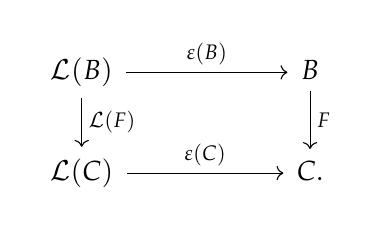
\begin{tikzpicture}
        \node {\begin{tikzcd}[column sep=20mm]
            \CC\LL(B)\ar[r,"\varepsilon(B)"]\ar[d,"\CC\LL(F)"] & B\ar[d,"F"]\\
            \CC\LL(C)\ar[r,"\varepsilon(C)"] & C.
          \end{tikzcd}};
      \end{tikzpicture}
    \]

    That is, we have to check that $\varepsilon(C)\circ \CC\LL(F) = F \circ \varepsilon(B)$. This is trivially checked on objects. On arrows, we have to check that, for every $f = \lambda x^a.\varphi(x^a) \in \CC\LL(F) $ we have that $\varepsilon(C)\circ \CC\LL(F) (f)= F \circ \varepsilon(B)(f)$.

    \begin{itemize}
    \item  $F \circ \varepsilon(B)(f) = F(g)$ where $g$ is the only function  such that$$gx^a = \varphi(x^a) \in \mathcal B[x^a].$$
    \item $\CC\LL(F) = \lambda x^{F(a)}.F_{x^a\to F(x^a)} \left ( \varphi(x^a)\right )$. Then we have that $\varepsilon(C)\circ \CC\LL(F) = h$ where $h$ is the only function such that $$h\circ F(x^a) = F_{x^a\to (x^{F(a)})}\left ( \varphi(x^a)\right ).$$
    \end{itemize}
    We finish by considering that $F(g)\circ F(x^a) = F_{x^a\to (x^{F(a)})}(g \circ x^a) = F_{x^a\to (x^{F(a)})}(\varphi(x^a)) $, and therefore $\varepsilon$ is natural.\\

  \item[\fbox{$ 1_{\mathcal A}\cong \LL \CC $}] We start by studying the language $\LL\CC(L)$, given $L$ a language. Is easy to check that the types in both languages are the same.\\

    Remember that arrows $f:a\to b$ in $\CC(L)$ are closed terms $\lambda x^a.f(x)$ of type $a\to b$. Finally, every term $M$ of type $A$ in $\LL\CC(L)$ has the form $\varphi(x^1,...,x^n): 1 \to A$, where $\varphi(x^{t_1},...,x^{t_n})$ is an arrow in $\CC(L)$ dependent on some indeterminates, thus $M =\lambda z^1.m(x^1,...,x^n)$\footnote{Here we are identifying $\CC(L)[x_1,...,x_n]$ with $\CC(L(x_1,...,x_n))$}.\\


    We define the unit $\eta$ of the adjoint equivalence similarly.
    \begin{itemize}
    \item For every $L\in \LC$ and every type $t\in L$ we have that $\eta(L)(t) = t$.
    \item For every term $\lamba z^1.\varphi (x_1^{t_1},...,x_n^{t_n})$, were every $x_i^{t_i}$ represents a free variable, to $\lambda z^1. \varphi (x_1^{t_1},...,x_n^{t_n}).$
    \end{itemize}


    It is easy to check that $\eta(L)$ is a $\lambda$-morphism. To check that it is an isomorphism on home sets we can construct the inverse arrow $\nu(L)$

    \begin{itemize}
    \item  $\nu(L)(t) = t$ for every type $t \in \LL\CC(L).$
    \item  Let $\lambda z^1.\varphi(x_1,...,x_n)$ be a term in $\LL\CC(L)$ with $x_1,...,x_n$ as free variables. We define $\nu(L)(f)= f* = \varphi(x_1,...,x_n)$.  
    \end{itemize}

    Naturality is checked as in the first part of the proof, developing in each equality term. 
  \end{enumerate}
\end{proof}


% \subsubsection{Deduction Theorem}
% We proceed with the tating that an arrow $f:\top \to A$ does exists in our deduction system. It can be deduced in both positive (without $\lor$ and $\bot$) an intuitionistic calculus that is $A \land B\vdash C$ then $A \vdash C\to B$. This theorem is more interesting to state in the new optics of deduction systems:
% \begin{theorem}[Proposition 2.1, \cite{lambek1988introduction}]
%   In a positive  calculus, if assuming the existence of an arrow $f:\top \to A$ implies the existence of an arrow $g: B\to C$, then there exists an arrow $h: A\land B\to C$ that does not depend on $f$.
% \end{theorem}

% \begin{sproof}
%   In a similar fashion of the Church-Rosser Theorem, it is solved by induction in the last rule used in the deduction.
% \end{sproof}


% As we have seen, a category is a deductive system with added structure.




\appendix

\chapter{Haskell}\label{aped.A}
\section*{BNF Notation in Haskell} \label{def:BN-Notation}


\section*{Acknowledgements}



%-----------------------------------------------------------------------------
%	BIBLIOGRAPHY
%-----------------------------------------------------------------------------
\medskip
\addcontentsline{toc}{chapter}{Bibliography}
\printbibliography

\end{document}  
